%%%% relatorio_pt.tex
%%%% Relatório do trabalho feito, no modelo IJCAI--ECAI 26 (REV-065, escrito a preto).
%%%% A proposta anterior está na etiqueta git proposta-pt-v1 (PDF em proposta_pt.pdf).
%%%% Compilar a partir de latex/.

\typeout{Project report using IJCAI--ECAI 26 formatting}

\documentclass{article}
\pdfpagewidth=8.5in
\pdfpageheight=11in

\usepackage{FormattingGuidelines-IJCAI-ECAI-26/ijcai26}
\usepackage{times}
\usepackage{soul}
\usepackage{url}
\usepackage[hidelinks]{hyperref}
\usepackage[utf8]{inputenc}
\usepackage[small]{caption}
\usepackage{graphicx}
\usepackage{tikz}
\usepackage{placeins}
\usetikzlibrary{positioning,arrows.meta}
\usepackage{amsmath}
\usepackage{booktabs}
\usepackage{xcolor}

\renewcommand{\figurename}{Figura}
\renewcommand{\tablename}{Tabela}

% Para marcar revisões: \revtext{revNNN}{texto}, com a cor do REVISION_LOG.md. Em REV-072, a pedido, todo o texto está a preto.
\newcommand{\revtext}[2]{{\color{#1}#2}}
% Número com vírgula decimal em modo matemático (sinal de menos correto).
\newcommand{\ptnum}[1]{{\mathcode`\,="013B\relax$#1$}}

% Números gerados por código (ais.cli.build_*); não editar à mão.
% Gerado por ais.cli.build_final_results em 2026-11-24T00:35:51+00:00 (commit 9ab2e46cf).
% NÃO EDITAR À MÃO: volta a gerar-se a partir de results/baseline_frozen/final_results.json.
\newcommand{\resDadosLinhas}{1\,026\,279}
\newcommand{\resDadosViagens}{123}
\newcommand{\resDadosLinhasTreino}{713\,854}
\newcommand{\resDadosViagensTreino}{87}
\newcommand{\resDadosPercPesca}{75,4\,\%}
\newcommand{\resPrepCoincide}{99,9997\,\%}
\newcommand{\resPrepBearingMediana}{1,1}
\newcommand{\resModParametros}{21\,761}
\newcommand{\resModCampo}{13}
\newcommand{\resModParamA}{1\,152}
\newcommand{\resModParamB}{10\,304}
\newcommand{\resModParamC}{10\,272}
\newcommand{\resModParamD}{33}
\newcommand{\resTrViagens}{87}
\newcommand{\resTrPontos}{713\,854}
\newcommand{\resTrEpocas}{300}
\newcommand{\resTrMaxEpocas}{300}
\newcommand{\resTrSegundos}{19}
\newcommand{\resTrSegPorEpoca}{2,8}
\newcommand{\resTrOrcamentoMin}{25}
\newcommand{\resTrSemente}{42}
\newcommand{\resTrTorch}{2.15.0}
\newcommand{\resSelEpoca}{162}
\newcommand{\resSelLimiar}{0,65}
\newcommand{\resSelNCand}{300}
\newcommand{\resSelViagens}{18}
\newcommand{\resSelPontos}{103\,409}
\newcommand{\resSelPerdaTeste}{0,185}
\newcommand{\resSelPerdaTesteMax}{0,342}
\newcommand{\resSelPerdaTreino}{0,149}
\newcommand{\resSelGrelhaMin}{0,05}
\newcommand{\resSelGrelhaMax}{0,95}
\newcommand{\resTreinoPontos}{713\,854}
\newcommand{\resTreinoErros}{46\,312}
\newcommand{\resTreinoAcc}{93,5\,\%}
\newcommand{\resTreinoAccMaj}{75,4\,\%}
\newcommand{\resTreinoPercPesca}{75,4\,\%}
\newcommand{\resTreinoNavReal}{175\,584}
\newcommand{\resTreinoPescaReal}{538\,270}
\newcommand{\resTreinoNavPrec}{0,832}
\newcommand{\resTreinoNavSens}{0,923}
\newcommand{\resTreinoNavF}{0,875}
\newcommand{\resTreinoNavIoU}{0,778}
\newcommand{\resTreinoPescaPrec}{0,974}
\newcommand{\resTreinoPescaSens}{0,939}
\newcommand{\resTreinoPescaF}{0,956}
\newcommand{\resTreinoPescaIoU}{0,916}
\newcommand{\resTreinoTN}{162\,072}
\newcommand{\resTreinoFP}{13\,512}
\newcommand{\resTreinoFN}{32\,800}
\newcommand{\resTreinoTP}{505\,470}
\newcommand{\resTestePontos}{103\,409}
\newcommand{\resTesteErros}{5\,502}
\newcommand{\resTesteAcc}{94,7\,\%}
\newcommand{\resTesteAccMaj}{61,2\,\%}
\newcommand{\resTestePercPesca}{61,2\,\%}
\newcommand{\resTesteNavReal}{40\,122}
\newcommand{\resTestePescaReal}{63\,287}
\newcommand{\resTesteNavPrec}{0,900}
\newcommand{\resTesteNavSens}{0,971}
\newcommand{\resTesteNavF}{0,934}
\newcommand{\resTesteNavIoU}{0,876}
\newcommand{\resTestePescaPrec}{0,981}
\newcommand{\resTestePescaSens}{0,931}
\newcommand{\resTestePescaF}{0,955}
\newcommand{\resTestePescaIoU}{0,915}
\newcommand{\resTesteTN}{38\,964}
\newcommand{\resTesteFP}{1\,158}
\newcommand{\resTesteFN}{4\,344}
\newcommand{\resTesteTP}{58\,943}
\newcommand{\resTesteViagMin}{74,0\,\%}
\newcommand{\resTesteViagMed}{97,1\,\%}
\newcommand{\resTesteViagMax}{99,8\,\%}
\newcommand{\resTestePiorViagem}{\texttt{220006000-2}}
\newcommand{\resTesteNViagNaoSuperam}{0}

% Gerado por ais.cli.build_window_results em 2026-11-24T00:36:00+00:00 (commit 9ab2e46cf).
% NÃO EDITAR À MÃO: volta a gerar-se a partir de results/windows_final/final_results_windows.json.
% Prefixos: Bs = baseline (viagem completa); JZ = J0 (0 % de sobreposição); JC = J50 (50 %).
\newcommand{\resBsTreinoPontos}{713\,854}
\newcommand{\resBsTreinoErros}{46\,312}
\newcommand{\resBsTreinoAcc}{93,5\,\%}
\newcommand{\resBsTreinoAccMaj}{75,4\,\%}
\newcommand{\resBsTreinoNavPrec}{0,832}
\newcommand{\resBsTreinoNavSens}{0,923}
\newcommand{\resBsTreinoNavF}{0,875}
\newcommand{\resBsTreinoNavIoU}{0,778}
\newcommand{\resBsTreinoPescaPrec}{0,974}
\newcommand{\resBsTreinoPescaSens}{0,939}
\newcommand{\resBsTreinoPescaF}{0,956}
\newcommand{\resBsTreinoPescaIoU}{0,916}
\newcommand{\resBsTreinoNavReal}{175\,584}
\newcommand{\resBsTreinoPescaReal}{538\,270}
\newcommand{\resBsTreinoTN}{162\,072}
\newcommand{\resBsTreinoFP}{13\,512}
\newcommand{\resBsTreinoFN}{32\,800}
\newcommand{\resBsTreinoTP}{505\,470}
\newcommand{\resBsTestePontos}{103\,409}
\newcommand{\resBsTesteErros}{5\,502}
\newcommand{\resBsTesteAcc}{94,7\,\%}
\newcommand{\resBsTesteAccMaj}{61,2\,\%}
\newcommand{\resBsTesteNavPrec}{0,900}
\newcommand{\resBsTesteNavSens}{0,971}
\newcommand{\resBsTesteNavF}{0,934}
\newcommand{\resBsTesteNavIoU}{0,876}
\newcommand{\resBsTestePescaPrec}{0,981}
\newcommand{\resBsTestePescaSens}{0,931}
\newcommand{\resBsTestePescaF}{0,955}
\newcommand{\resBsTestePescaIoU}{0,915}
\newcommand{\resBsTesteNavReal}{40\,122}
\newcommand{\resBsTestePescaReal}{63\,287}
\newcommand{\resBsTesteTN}{38\,964}
\newcommand{\resBsTesteFP}{1\,158}
\newcommand{\resBsTesteFN}{4\,344}
\newcommand{\resBsTesteTP}{58\,943}
\newcommand{\resBsSegPescaNRef}{18}
\newcommand{\resBsSegPescaNPred}{358}
\newcommand{\resBsSegPescaNPar}{6}
\newcommand{\resBsSegPescaPrec}{0,017}
\newcommand{\resBsSegPescaSens}{0,333}
\newcommand{\resBsSegPescaF}{0,032}
\newcommand{\resBsSegPescaIoUMed}{0,707}
\newcommand{\resBsSegPescaIniMed}{8439}
\newcommand{\resBsSegPescaFimMed}{100}
\newcommand{\resBsSegPescaFrag}{19,89}
\newcommand{\resBsSegNavNRef}{36}
\newcommand{\resBsSegNavNPred}{376}
\newcommand{\resBsSegNavNPar}{31}
\newcommand{\resBsSegNavPrec}{0,082}
\newcommand{\resBsSegNavSens}{0,861}
\newcommand{\resBsSegNavF}{0,150}
\newcommand{\resBsSegNavIoUMed}{0,934}
\newcommand{\resBsSegNavIniMed}{0}
\newcommand{\resBsSegNavFimMed}{31}
\newcommand{\resBsSegNavFrag}{10,44}
\newcommand{\resBsEpoca}{162}
\newcommand{\resBsLimiar}{0,65}
\newcommand{\resBsPassos}{87}
\newcommand{\resBsPassosTotal}{26\,100}
\newcommand{\resBsEpocas}{300}
\newcommand{\resBsSegundos}{19}
\newcommand{\resJZL}{64}
\newcommand{\resJZSobrep}{0\,\%}
\newcommand{\resJZPasso}{64}
\newcommand{\resJZLote}{32}
\newcommand{\resJZJanelas}{11\,201}
\newcommand{\resJZJanelasCurtas}{87}
\newcommand{\resJZPassos}{351}
\newcommand{\resJZPassosTotal}{105\,300}
\newcommand{\resJZEpocas}{300}
\newcommand{\resJZSegundos}{10}
\newcommand{\resJZSegPorEpoca}{1,6}
\newcommand{\resJZOrcamentoMin}{45}
\newcommand{\resJZEpoca}{8}
\newcommand{\resJZLimiar}{0,60}
\newcommand{\resJZNaoConvergiu}{não}
\newcommand{\resJZJanelasTeste}{1\,622}
\newcommand{\resJZPerdaTeste}{0,212}
\newcommand{\resJZPerdaTesteMax}{0,788}
\newcommand{\resJZPerdaTreino}{0,181}
\newcommand{\resJZViagMelhor}{7}
\newcommand{\resJZViagIgual}{0}
\newcommand{\resJZViagPior}{11}
\newcommand{\resJZViagDifMed}{-0,2}
\newcommand{\resJZTreinoPontos}{713\,854}
\newcommand{\resJZTreinoErros}{51\,953}
\newcommand{\resJZTreinoAcc}{92,7\,\%}
\newcommand{\resJZTreinoAccMaj}{75,4\,\%}
\newcommand{\resJZTreinoNavPrec}{0,813}
\newcommand{\resJZTreinoNavSens}{0,915}
\newcommand{\resJZTreinoNavF}{0,861}
\newcommand{\resJZTreinoNavIoU}{0,756}
\newcommand{\resJZTreinoPescaPrec}{0,971}
\newcommand{\resJZTreinoPescaSens}{0,931}
\newcommand{\resJZTreinoPescaF}{0,951}
\newcommand{\resJZTreinoPescaIoU}{0,906}
\newcommand{\resJZTreinoNavReal}{175\,584}
\newcommand{\resJZTreinoPescaReal}{538\,270}
\newcommand{\resJZTreinoTN}{160\,660}
\newcommand{\resJZTreinoFP}{14\,924}
\newcommand{\resJZTreinoFN}{37\,029}
\newcommand{\resJZTreinoTP}{501\,241}
\newcommand{\resJZTestePontos}{103\,409}
\newcommand{\resJZTesteErros}{6\,775}
\newcommand{\resJZTesteAcc}{93,4\,\%}
\newcommand{\resJZTesteAccMaj}{61,2\,\%}
\newcommand{\resJZTesteNavPrec}{0,905}
\newcommand{\resJZTesteNavSens}{0,929}
\newcommand{\resJZTesteNavF}{0,917}
\newcommand{\resJZTesteNavIoU}{0,846}
\newcommand{\resJZTestePescaPrec}{0,954}
\newcommand{\resJZTestePescaSens}{0,938}
\newcommand{\resJZTestePescaF}{0,946}
\newcommand{\resJZTestePescaIoU}{0,898}
\newcommand{\resJZTesteNavReal}{40\,122}
\newcommand{\resJZTestePescaReal}{63\,287}
\newcommand{\resJZTesteTN}{37\,257}
\newcommand{\resJZTesteFP}{2\,865}
\newcommand{\resJZTesteFN}{3\,910}
\newcommand{\resJZTesteTP}{59\,377}
\newcommand{\resJZSegPescaNRef}{18}
\newcommand{\resJZSegPescaNPred}{377}
\newcommand{\resJZSegPescaNPar}{6}
\newcommand{\resJZSegPescaPrec}{0,016}
\newcommand{\resJZSegPescaSens}{0,333}
\newcommand{\resJZSegPescaF}{0,030}
\newcommand{\resJZSegPescaIoUMed}{0,734}
\newcommand{\resJZSegPescaIniMed}{2986}
\newcommand{\resJZSegPescaFimMed}{454}
\newcommand{\resJZSegPescaFrag}{20,94}
\newcommand{\resJZSegNavNRef}{36}
\newcommand{\resJZSegNavNPred}{395}
\newcommand{\resJZSegNavNPar}{32}
\newcommand{\resJZSegNavPrec}{0,081}
\newcommand{\resJZSegNavSens}{0,889}
\newcommand{\resJZSegNavF}{0,148}
\newcommand{\resJZSegNavIoUMed}{0,901}
\newcommand{\resJZSegNavIniMed}{0}
\newcommand{\resJZSegNavFimMed}{30}
\newcommand{\resJZSegNavFrag}{10,97}
\newcommand{\resJZTesteViagMin}{42,0\,\%}
\newcommand{\resJZTesteViagMed}{96,2\,\%}
\newcommand{\resJZTesteViagMax}{99,6\,\%}
\newcommand{\resJZTesteNViagNaoSuperam}{2}
\newcommand{\resJCL}{64}
\newcommand{\resJCSobrep}{50\,\%}
\newcommand{\resJCPasso}{32}
\newcommand{\resJCLote}{32}
\newcommand{\resJCJanelas}{22\,265}
\newcommand{\resJCJanelasCurtas}{86}
\newcommand{\resJCPassos}{696}
\newcommand{\resJCPassosTotal}{208\,800}
\newcommand{\resJCEpocas}{300}
\newcommand{\resJCSegundos}{21}
\newcommand{\resJCSegPorEpoca}{3,6}
\newcommand{\resJCOrcamentoMin}{45}
\newcommand{\resJCEpoca}{4}
\newcommand{\resJCLimiar}{0,75}
\newcommand{\resJCNaoConvergiu}{não}
\newcommand{\resJCJanelasTeste}{3\,221}
\newcommand{\resJCPerdaTeste}{0,210}
\newcommand{\resJCPerdaTesteMax}{0,929}
\newcommand{\resJCPerdaTreino}{0,174}
\newcommand{\resJCViagMelhor}{5}
\newcommand{\resJCViagIgual}{0}
\newcommand{\resJCViagPior}{13}
\newcommand{\resJCViagDifMed}{-1,1}
\newcommand{\resJCTreinoPontos}{713\,854}
\newcommand{\resJCTreinoErros}{51\,414}
\newcommand{\resJCTreinoAcc}{92,8\,\%}
\newcommand{\resJCTreinoAccMaj}{75,4\,\%}
\newcommand{\resJCTreinoNavPrec}{0,811}
\newcommand{\resJCTreinoNavSens}{0,923}
\newcommand{\resJCTreinoNavF}{0,863}
\newcommand{\resJCTreinoNavIoU}{0,759}
\newcommand{\resJCTreinoPescaPrec}{0,974}
\newcommand{\resJCTreinoPescaSens}{0,930}
\newcommand{\resJCTreinoPescaF}{0,951}
\newcommand{\resJCTreinoPescaIoU}{0,907}
\newcommand{\resJCTreinoNavReal}{175\,584}
\newcommand{\resJCTreinoPescaReal}{538\,270}
\newcommand{\resJCTreinoTN}{161\,995}
\newcommand{\resJCTreinoFP}{13\,589}
\newcommand{\resJCTreinoFN}{37\,825}
\newcommand{\resJCTreinoTP}{500\,445}
\newcommand{\resJCTestePontos}{103\,409}
\newcommand{\resJCTesteErros}{6\,464}
\newcommand{\resJCTesteAcc}{93,7\,\%}
\newcommand{\resJCTesteAccMaj}{61,2\,\%}
\newcommand{\resJCTesteNavPrec}{0,910}
\newcommand{\resJCTesteNavSens}{0,931}
\newcommand{\resJCTesteNavF}{0,920}
\newcommand{\resJCTesteNavIoU}{0,852}
\newcommand{\resJCTestePescaPrec}{0,956}
\newcommand{\resJCTestePescaSens}{0,942}
\newcommand{\resJCTestePescaF}{0,949}
\newcommand{\resJCTestePescaIoU}{0,902}
\newcommand{\resJCTesteNavReal}{40\,122}
\newcommand{\resJCTestePescaReal}{63\,287}
\newcommand{\resJCTesteTN}{37\,358}
\newcommand{\resJCTesteFP}{2\,764}
\newcommand{\resJCTesteFN}{3\,700}
\newcommand{\resJCTesteTP}{59\,587}
\newcommand{\resJCSegPescaNRef}{18}
\newcommand{\resJCSegPescaNPred}{303}
\newcommand{\resJCSegPescaNPar}{5}
\newcommand{\resJCSegPescaPrec}{0,017}
\newcommand{\resJCSegPescaSens}{0,278}
\newcommand{\resJCSegPescaF}{0,031}
\newcommand{\resJCSegPescaIoUMed}{0,721}
\newcommand{\resJCSegPescaIniMed}{5402}
\newcommand{\resJCSegPescaFimMed}{3784}
\newcommand{\resJCSegPescaFrag}{16,83}
\newcommand{\resJCSegNavNRef}{36}
\newcommand{\resJCSegNavNPred}{318}
\newcommand{\resJCSegNavNPar}{33}
\newcommand{\resJCSegNavPrec}{0,104}
\newcommand{\resJCSegNavSens}{0,917}
\newcommand{\resJCSegNavF}{0,186}
\newcommand{\resJCSegNavIoUMed}{0,910}
\newcommand{\resJCSegNavIniMed}{0}
\newcommand{\resJCSegNavFimMed}{31}
\newcommand{\resJCSegNavFrag}{8,83}
\newcommand{\resJCTesteViagMin}{66,4\,\%}
\newcommand{\resJCTesteViagMed}{95,8\,\%}
\newcommand{\resJCTesteViagMax}{98,8\,\%}
\newcommand{\resJCTesteNViagNaoSuperam}{1}
\newcommand{\resBsTesteViagMed}{97,1\,\%}
\newcommand{\resJCPassosVezes}{2,0}

% Gerado por ais.cli.build_validation_results em 2026-11-24T00:32:10+00:00 (medição final, commit 9ab2e46cf).
% NÃO EDITAR À MÃO: volta a gerar-se a partir de results/final_validation/final_validation.json.
% Prefixos: Va = validation (e Va...Teste = test do mesmo modelo); VaT = segmentos do test.
\newcommand{\resVaModelo}{a referência (viagem completa)}
\newcommand{\resVaEpoca}{162}
\newcommand{\resVaLimiar}{0,65}
\newcommand{\resVaPontos}{209\,016}
\newcommand{\resVaViagens}{18}
\newcommand{\resVaPercPesca}{83,2\,\%}
\newcommand{\resVaFMedioBs}{0,945}
\newcommand{\resVaAccTesteBs}{94,7\,\%}
\newcommand{\resVaFMedioJC}{0,934}
\newcommand{\resVaAccTesteJC}{93,7\,\%}
\newcommand{\resVaFMedioJZ}{0,931}
\newcommand{\resVaAccTesteJZ}{93,4\,\%}
\newcommand{\resVaValidPontos}{209\,016}
\newcommand{\resVaValidErros}{11\,662}
\newcommand{\resVaValidAcc}{94,4\,\%}
\newcommand{\resVaValidAccMaj}{83,2\,\%}
\newcommand{\resVaValidNavPrec}{0,760}
\newcommand{\resVaValidNavSens}{0,976}
\newcommand{\resVaValidNavF}{0,854}
\newcommand{\resVaValidNavIoU}{0,746}
\newcommand{\resVaValidPescaPrec}{0,995}
\newcommand{\resVaValidPescaSens}{0,938}
\newcommand{\resVaValidPescaF}{0,965}
\newcommand{\resVaValidPescaIoU}{0,933}
\newcommand{\resVaValidNavReal}{35\,052}
\newcommand{\resVaValidPescaReal}{173\,964}
\newcommand{\resVaValidTN}{34\,226}
\newcommand{\resVaValidFP}{826}
\newcommand{\resVaValidFN}{10\,836}
\newcommand{\resVaValidTP}{163\,128}
\newcommand{\resVaTestePontos}{103\,409}
\newcommand{\resVaTesteErros}{5\,502}
\newcommand{\resVaTesteAcc}{94,7\,\%}
\newcommand{\resVaTesteAccMaj}{61,2\,\%}
\newcommand{\resVaTesteNavPrec}{0,900}
\newcommand{\resVaTesteNavSens}{0,971}
\newcommand{\resVaTesteNavF}{0,934}
\newcommand{\resVaTesteNavIoU}{0,876}
\newcommand{\resVaTestePescaPrec}{0,981}
\newcommand{\resVaTestePescaSens}{0,931}
\newcommand{\resVaTestePescaF}{0,955}
\newcommand{\resVaTestePescaIoU}{0,915}
\newcommand{\resVaTesteNavReal}{40\,122}
\newcommand{\resVaTestePescaReal}{63\,287}
\newcommand{\resVaTesteTN}{38\,964}
\newcommand{\resVaTesteFP}{1\,158}
\newcommand{\resVaTesteFN}{4\,344}
\newcommand{\resVaTesteTP}{58\,943}
\newcommand{\resVaSegPescaNRef}{18}
\newcommand{\resVaSegPescaNPred}{486}
\newcommand{\resVaSegPescaNPar}{7}
\newcommand{\resVaSegPescaPrec}{0,014}
\newcommand{\resVaSegPescaSens}{0,389}
\newcommand{\resVaSegPescaF}{0,028}
\newcommand{\resVaSegPescaIoUMed}{0,590}
\newcommand{\resVaSegPescaIniMed}{460}
\newcommand{\resVaSegPescaFimMed}{22690}
\newcommand{\resVaSegPescaFrag}{27,00}
\newcommand{\resVaSegNavNRef}{35}
\newcommand{\resVaSegNavNPred}{502}
\newcommand{\resVaSegNavNPar}{32}
\newcommand{\resVaSegNavPrec}{0,064}
\newcommand{\resVaSegNavSens}{0,914}
\newcommand{\resVaSegNavF}{0,119}
\newcommand{\resVaSegNavIoUMed}{0,930}
\newcommand{\resVaSegNavIniMed}{0}
\newcommand{\resVaSegNavFimMed}{80}
\newcommand{\resVaSegNavFrag}{14,34}
\newcommand{\resVaTSegPescaNRef}{18}
\newcommand{\resVaTSegPescaNPred}{358}
\newcommand{\resVaTSegPescaNPar}{6}
\newcommand{\resVaTSegPescaPrec}{0,017}
\newcommand{\resVaTSegPescaSens}{0,333}
\newcommand{\resVaTSegPescaF}{0,032}
\newcommand{\resVaTSegPescaIoUMed}{0,707}
\newcommand{\resVaTSegPescaIniMed}{8439}
\newcommand{\resVaTSegPescaFimMed}{100}
\newcommand{\resVaTSegPescaFrag}{19,89}
\newcommand{\resVaTSegNavNRef}{36}
\newcommand{\resVaTSegNavNPred}{376}
\newcommand{\resVaTSegNavNPar}{31}
\newcommand{\resVaTSegNavPrec}{0,082}
\newcommand{\resVaTSegNavSens}{0,861}
\newcommand{\resVaTSegNavF}{0,150}
\newcommand{\resVaTSegNavIoUMed}{0,934}
\newcommand{\resVaTSegNavIniMed}{0}
\newcommand{\resVaTSegNavFimMed}{31}
\newcommand{\resVaTSegNavFrag}{10,44}
\newcommand{\resVaViagMin}{40,4\,\%}
\newcommand{\resVaViagMed}{98,2\,\%}
\newcommand{\resVaViagMax}{99,7\,\%}
\newcommand{\resVaPiorViagem}{\texttt{219020187-4}}
\newcommand{\resVaNViagNaoSuperam}{1}

% Gerado por ais.cli.build_postproc_results a partir de results/postproc_validation/postproc_validation.json
% (execução única 2026-11-25T19:45:19+00:00, commit afe1c64cc). NÃO EDITAR À MÃO.
% Prefixos: PpAntes/PpDepois = por ponto; PpASeg/PpDSeg = por segmento antes/depois.
\newcommand{\resPpAntesPontos}{209\,016}
\newcommand{\resPpAntesErros}{11\,662}
\newcommand{\resPpAntesAcc}{94,4\,\%}
\newcommand{\resPpAntesAccMaj}{83,2\,\%}
\newcommand{\resPpAntesNavPrec}{0,760}
\newcommand{\resPpAntesNavSens}{0,976}
\newcommand{\resPpAntesNavF}{0,854}
\newcommand{\resPpAntesNavIoU}{0,746}
\newcommand{\resPpAntesPescaPrec}{0,995}
\newcommand{\resPpAntesPescaSens}{0,938}
\newcommand{\resPpAntesPescaF}{0,965}
\newcommand{\resPpAntesPescaIoU}{0,933}
\newcommand{\resPpAntesNavReal}{35\,052}
\newcommand{\resPpAntesPescaReal}{173\,964}
\newcommand{\resPpAntesTN}{34\,226}
\newcommand{\resPpAntesFP}{826}
\newcommand{\resPpAntesFN}{10\,836}
\newcommand{\resPpAntesTP}{163\,128}
\newcommand{\resPpDepoisPontos}{209\,016}
\newcommand{\resPpDepoisErros}{11\,418}
\newcommand{\resPpDepoisAcc}{94,5\,\%}
\newcommand{\resPpDepoisAccMaj}{83,2\,\%}
\newcommand{\resPpDepoisNavPrec}{0,763}
\newcommand{\resPpDepoisNavSens}{0,978}
\newcommand{\resPpDepoisNavF}{0,857}
\newcommand{\resPpDepoisNavIoU}{0,750}
\newcommand{\resPpDepoisPescaPrec}{0,995}
\newcommand{\resPpDepoisPescaSens}{0,939}
\newcommand{\resPpDepoisPescaF}{0,966}
\newcommand{\resPpDepoisPescaIoU}{0,935}
\newcommand{\resPpDepoisNavReal}{35\,052}
\newcommand{\resPpDepoisPescaReal}{173\,964}
\newcommand{\resPpDepoisTN}{34\,288}
\newcommand{\resPpDepoisFP}{764}
\newcommand{\resPpDepoisFN}{10\,654}
\newcommand{\resPpDepoisTP}{163\,310}
\newcommand{\resPpASegPescaNRef}{18}
\newcommand{\resPpASegPescaNPred}{486}
\newcommand{\resPpASegPescaNPar}{7}
\newcommand{\resPpASegPescaPrec}{0,014}
\newcommand{\resPpASegPescaSens}{0,389}
\newcommand{\resPpASegPescaF}{0,028}
\newcommand{\resPpASegPescaIoUMed}{0,590}
\newcommand{\resPpASegPescaIniMed}{460}
\newcommand{\resPpASegPescaFimMed}{22690}
\newcommand{\resPpASegPescaFrag}{27,00}
\newcommand{\resPpASegNavNRef}{35}
\newcommand{\resPpASegNavNPred}{502}
\newcommand{\resPpASegNavNPar}{32}
\newcommand{\resPpASegNavPrec}{0,064}
\newcommand{\resPpASegNavSens}{0,914}
\newcommand{\resPpASegNavF}{0,119}
\newcommand{\resPpASegNavIoUMed}{0,930}
\newcommand{\resPpASegNavIniMed}{0}
\newcommand{\resPpASegNavFimMed}{80}
\newcommand{\resPpASegNavFrag}{14,34}
\newcommand{\resPpDSegPescaNRef}{18}
\newcommand{\resPpDSegPescaNPred}{255}
\newcommand{\resPpDSegPescaNPar}{9}
\newcommand{\resPpDSegPescaPrec}{0,035}
\newcommand{\resPpDSegPescaSens}{0,500}
\newcommand{\resPpDSegPescaF}{0,066}
\newcommand{\resPpDSegPescaIoUMed}{0,623}
\newcommand{\resPpDSegPescaIniMed}{469}
\newcommand{\resPpDSegPescaFimMed}{22655}
\newcommand{\resPpDSegPescaFrag}{14,17}
\newcommand{\resPpDSegNavNRef}{35}
\newcommand{\resPpDSegNavNPred}{272}
\newcommand{\resPpDSegNavNPar}{34}
\newcommand{\resPpDSegNavPrec}{0,125}
\newcommand{\resPpDSegNavSens}{0,971}
\newcommand{\resPpDSegNavF}{0,221}
\newcommand{\resPpDSegNavIoUMed}{0,925}
\newcommand{\resPpDSegNavIniMed}{0}
\newcommand{\resPpDSegNavFimMed}{54}
\newcommand{\resPpDSegNavFrag}{7,77}
\newcommand{\resPpMudam}{784}
\newcommand{\resPpNavParaPesca}{452}
\newcommand{\resPpPescaParaNav}{332}
\newcommand{\resPpCorrigidos}{514}
\newcommand{\resPpEstragados}{270}
\newcommand{\resPpPercMudam}{0,38\,\%}
\newcommand{\resPpErrosMenos}{244}

% Gerado por ais.cli.build_postproc_results --first-version-only a partir de results/postproc_validation/postproc_validation.json
% (execução única 2026-11-25T19:45:19+00:00, commit afe1c64cc). NÃO EDITAR À MÃO.
\newcommand{\resPpViJanela}{13}
\newcommand{\resPpViDepoisAcc}{94,5\,\%}
\newcommand{\resPpViSegPescaNPred}{255}
\newcommand{\resPpViSegPescaF}{0,066}
\newcommand{\resPpViViagMelhoram}{12}
\newcommand{\resPpViViagPioram}{6}

% Gerado por ais.cli.build_window_analysis_macros a partir de results/postproc_window_analysis/
% (análise do test de 2026-11-25T20:00:19+00:00, janela de 301 pontos). NÃO EDITAR À MÃO.
\newcommand{\resBuTesteBlocos}{373}
\newcommand{\resBuTesteErros}{5\,502}
\newcommand{\resBuTesteMedia}{14,8}
\newcommand{\resBuTesteMediana}{5}
\newcommand{\resBuTesteNoventa}{37}
\newcommand{\resBuTesteMaximo}{286}
\newcommand{\resBuTesteNavBlocos}{253}
\newcommand{\resBuTestePescaBlocos}{120}
\newcommand{\resBuTesteNavPercPontos}{79\,\%}
\newcommand{\resBuTesteRealNavMin}{127}
\newcommand{\resBuTesteRealPescaMin}{633}
\newcommand{\resBuTreinoRealNavMin}{102}
\newcommand{\resBuTreinoRealPescaMin}{584}
\newcommand{\resBuRemovePesca}{93}
\newcommand{\resBuRemoveNav}{45}
\newcommand{\resBuTesteBlocosCobertos}{93\,\%}
\newcommand{\resBuTestePontosCobertos}{59\,\%}


% Números de linha até à versão final.
\usepackage[switch]{lineno}
\linenumbers
\switchlinenumbers

\urlstyle{same}

% Required PDF metadata block. Keep unchanged.
\pdfinfo{
/TemplateVersion (IJCAI.2026.0)
}

\title{Segmenta\c{c}\~ao sem\^antica de trajet\'orias AIS para dete\c{c}\~ao de atividade de pesca usando janelas sobrepostas e p\'os-processamento temporal}

\author{
    Dinis Soveral Botelho Rosa
    \affiliations
    University of Coimbra / Department of Informatics Engineering
    \emails
    uc2024278343@student.uc.pt
}

% Figuras no sítio certo (REV-080): admitem-se mais figuras no topo de cada página.
\renewcommand{\dbltopfraction}{0.95}
\renewcommand{\textfraction}{0.05}
\setcounter{dbltopnumber}{4}
\setcounter{totalnumber}{6}
\begin{document}

\maketitle

\begin{abstract}
A pesca ilegal, não declarada e não regulamentada ameaça a sustentabilidade dos oceanos, e o \emph{Automatic Identification System} (AIS) permite acompanhar os navios à escala global. Este trabalho segmenta trajetórias AIS em pesca e navegação, com uma previsão por ponto, usando uma rede convolucional unidimensional pequena sobre \resDadosViagens{} viagens anotadas, e estuda o efeito de janelas sobrepostas e de um filtro temporal. No conjunto de teste, usado para escolher os modelos, as janelas com \resJCSobrep{} de sobreposição fragmentam menos do que as sem sobreposição, mas nenhuma variante com janelas supera em exatidão a rede aplicada à viagem completa. Na medição final, essa rede atinge \resVaValidAcc{} de exatidão por ponto (prever sempre a classe maioritária dá \resVaValidAccMaj{}), com uma segmentação muito fragmentada. Sobre as previsões dessa medição, testou-se um filtro gaussiano primeiro com \resPpViJanela{} pontos, com um ganho pequeno, e depois com \resPpJanela{}. Esta segunda janela reduz os segmentos de pesca previstos de \resPpASegPescaNPred{} para \resPpDSegPescaNPred{} (reais: \resPpASegPescaNRef{}) e sobe a exatidão para \resPpDepoisAcc{}, mas piora \resPpViagPioram{} das \resPpNViagens{} viagens. A interação entre sobreposição e filtro fica sem resposta, e a explicabilidade e o apoio à decisão não foram concluídos.
\end{abstract}

\section{Introdução}
\label{sec:introducao}
A pesca ilegal, não declarada e não regulamentada (IUU) ameaça a sustentabilidade dos oceanos. Agnew et al.~\shortcite{agnew2009} estimam que a pesca ilegal e não declarada cause perdas anuais entre 10 e 23,5 mil milhões de dólares, correspondentes a 11 a 26 milhões de toneladas de pescado; associa-se também à sobre-exploração e ao trabalho ilegal~\cite{chuaysi2020}. Fiscalizá-la exige saber onde e quando os navios pescam, algo difícil de obter só por inspeção, à escala da frota. O \emph{Automatic Identification System} (AIS) difunde a identidade, a posição, a velocidade e o rumo dos navios, com intervalos que vão de segundos a minutos conforme a manobra~\cite{natale2015}, e permite monitorizar a pesca à escala global~\cite{natale2015,kroodsma2018}.

O problema tratado é \textbf{classificar, ao longo de uma trajetória AIS, cada ponto como pesca ou navegação}, de modo que os intervalos resultantes sirvam a quem fiscaliza. A hipótese de partida era que as previsões ponto a ponto podem partir esses intervalos em muitos fragmentos, e que janelas sobrepostas e um pós-processamento temporal os podem tornar mais consistentes. Na linha da Inteligência Artificial Centrada no Humano (HCAI)~\cite{shneiderman2020}, o sistema destina-se a apoiar, e não a substituir, a decisão do inspetor.

\subsection{Objetivos}

O objetivo principal era desenvolver um sistema de segmentação semântica de trajetórias AIS que detete pesca de forma robusta e interpretável, combinando janelas sobrepostas e pós-processamento temporal, como apoio à decisão de inspetores (\emph{human-on-the-loop}, com o inspetor a supervisionar e a poder intervir). Os objetivos específicos eram:
\begin{enumerate}
\item construir um pré-processamento auditável, que recalcula as grandezas derivadas e seleciona as características, sem remover anomalias;
\item implementar e treinar uma CNN 1D que devolve uma probabilidade por ponto, primeiro sobre a viagem completa, como \emph{baseline}, e depois, com a mesma rede, sobre janelas com sobreposição;
\item conceber e avaliar um pós-processamento temporal que regularize as fronteiras dos segmentos, aplicado ao melhor dos modelos testados;
\item avaliar quantitativamente, por ponto e por segmento, e qualitativamente, com visualizações e casos de estudo;
\item incluir explicabilidade e confiança calibrada que sustentem a decisão do inspetor. Este objetivo não foi concluído nesta fase (Secção~\ref{sec:limitacoes}).
\end{enumerate}

\subsection{Perguntas de investigação e contribuições}

\textbf{RQ1:} em que medida as janelas sobrepostas reduzem a instabilidade das fronteiras face a janelas não sobrepostas? \textbf{RQ2:} em que medida o pós-processamento reduz a fragmentação e melhora a concordância com os segmentos anotados? \textbf{RQ3:} qual a interação entre sobreposição e pós-processamento?

Os critérios de sucesso definidos foram: (i) caracterizar quantitativamente o efeito das duas componentes face à CNN \emph{baseline}, aceitando como resultado válido que uma componente não traga ganho; (ii) produzir segmentações temporalmente estáveis; e (iii) fornecer justificações auditáveis para validação por um inspetor.

As contribuições são uma comparação entre uma CNN 1D sobre a viagem completa e a mesma rede sobre janelas, com e sem sobreposição, com os mesmos dados e o mesmo critério de seleção; evidência sobre o efeito de um filtro temporal aplicado ao melhor desses modelos; e um protocolo reprodutível, com conjuntos reservados, autorizações e registo de acessos.

\section{Trabalho relacionado}
\label{sec:relacionado}
Os primeiros métodos de identificação de pesca usaram modelos de Markov escondidos sobre dados do \emph{Vessel Monitoring System} (VMS): Peel e Good~\shortcite{peel2011} e Vermard et al.~\shortcite{vermard2010} distinguem estados como a pesca e a navegação a partir do movimento. Com o AIS, a escala aumentou: Natale et al.~\shortcite{natale2015} identificaram a pesca pelos perfis de velocidade e mapearam o esforço da frota sueca, e Kroodsma et al.~\shortcite{kroodsma2018} usaram redes convolucionais para mapear a pegada global da pesca.

Na segmentação de trajetórias, Soares Júnior et al.~\shortcite{soares2018} propuseram um método semi-supervisionado baseado em \emph{Minimum Description Length}. Wu et al.~\shortcite{wu2022}, o trabalho em que este projeto se baseia, classificam com uma floresta aleatória janelas sobrepostas de uma trajetória e juntam, por \emph{run-length encoding}, as janelas de pesca próximas, para detetar atividades de pesca completas.

Com aprendizagem profunda, Arasteh et al.~\shortcite{arasteh2020} classificam segmentos de atividade com uma CNN; Ferreira et al.~\shortcite{ferreira2022full} obtêm rótulos por agrupamento da geometria das rotas e treinam redes recorrentes; Hu et al.~\shortcite{hu2026} segmentam subtrajetórias sem supervisão, a partir de campos angulares de Gram, e preveem trajetórias; e o FishFormer~\cite{wang2026} combina atenção local e global para reconhecer quatro estados operacionais. Um problema próximo é identificar o tipo de navio de pesca, por exemplo com redes com atenção~\cite{cheng2025}.

Na dimensão humana, Shneiderman~\shortcite{shneiderman2020} defende combinar elevado controlo humano com elevada automação, em sistemas fiáveis, seguros e de confiança. Para apoiar quem decide, importa que as probabilidades sejam calibradas, o que muitas redes neuronais modernas não garantem~\cite{guo2017}, e métodos como o SHAP atribuem a cada característica a sua importância numa previsão~\cite{lundberg2017}.

Este trabalho não se compara numericamente com estes métodos: estuda, com uma só CNN pequena, o efeito das janelas, da sobreposição e de um filtro temporal na segmentação ponto a ponto, incluindo a sua fragmentação.

\section{Dados e preparação}
\label{sec:dados}
\subsection{Conjunto de dados}

Usa-se o conjunto público \emph{Detailed Labelled Fishing Trajectories from AIS} (Kaggle)~\cite{kaggleAIS}: \resDadosViagens{} trajetórias anotadas de navios de pesca, com \resDadosLinhas{} pontos e 13 colunas (12 atributos e o rótulo), entre as quais o identificador do navio e da viagem, o instante, a longitude e a latitude, as coordenadas projetadas, o rumo e a distância à costa. Wu et al.~\shortcite{wu2022} descrevem a origem destes dados: mensagens AIS de navios de pesca, da autoridade marítima dinamarquesa, entre 14 e 20 de novembro de 2021, das quais removeram posições duplicadas e fizeram a média das coordenadas com o mesmo instante, anotadas manualmente. O artigo refere 128 trajetórias e 1\,080\,220 pontos, com um intervalo médio de 10,63~s; o ficheiro público usado aqui tem menos trajetórias e menos pontos, diferença para a qual não se encontrou explicação (o nome do ficheiro e a página do repositório também indicam 128).

As cinco classes são agregadas num problema binário: pesca (\texttt{02-fishing} e \texttt{04-fishing}) e navegação (\texttt{01-sailing}, \texttt{03-sailing} e \texttt{05-sailing}). A pesca representa \resDadosPercPesca{} dos pontos de treino, \resTestePercPesca{} dos de teste e \resVaPercPesca{} dos de validação. Mantém-se o desequilíbrio natural e as viagens completas.

\subsection{Preparação}

Para cada viagem, a partir das coordenadas projetadas e do instante, recalculam-se o intervalo temporal (s), a distância entre pontos consecutivos (m), o rumo (graus, a partir do norte da grelha UTM), a variação de rumo com sinal, no intervalo $(-180,180]$ graus, e a velocidade (m/s). No treino, o intervalo, a distância e a variação de rumo coincidem com os valores originais em pelo menos \resPrepCoincide{} dos pares (tolerâncias de $10^{-6}$~s, $10^{-3}$~m e 1~grau); o rumo difere em \resPrepBearingMediana\textdegree{} (mediana), pela convergência dos meridianos. A distância à costa é usada tal como vem no conjunto, sem verificação externa.

Nenhuma linha é removida. Os saltos de posição, os intervalos longos e as inversões de rumo mantêm-se, por existirem em dados AIS reais; a robustez do modelo a essas anomalias não foi estudada em separado.

As entradas do modelo são quatro atributos (velocidade, variação de rumo, intervalo temporal e distância à costa), normalizados com a média e o desvio-padrão do treino. O primeiro ponto de cada viagem não tem velocidade, variação de rumo nem intervalo, e o segundo não tem variação de rumo; esses valores ficam a zero depois da normalização, e três indicadores de ausência distinguem-nos de um zero real. Os identificadores, os instantes e as coordenadas não são entradas. A preparação aplica-se a cada conjunto em separado e é verificada com testes sobre dados sintéticos.

\section{Método}
\label{sec:metodo}

\subsection{Visão geral}

O modelo é uma rede neuronal convolucional unidimensional (CNN 1D) que devolve, para cada ponto de uma viagem, a probabilidade de ele ser de pesca. A mesma rede é usada de duas formas: sobre a viagem completa, que serve de \textbf{\emph{baseline}}, o termo de comparação, e sobre janelas, sem e com sobreposição. Ao modelo escolhido aplica-se depois um filtro temporal que regulariza as previsões, e os segmentos de pesca e de navegação são os blocos de pontos seguidos com a mesma classe (Figura~\ref{fig:pipeline}).

\begin{center}
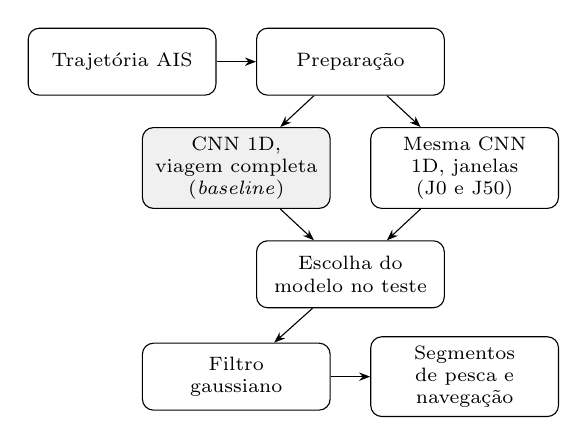
\begin{tikzpicture}[font=\scriptsize, >={Stealth[length=4pt]},
  box/.style={draw, rounded corners, align=center, minimum height=0.85cm, text width=2.15cm},
  ref/.style={box, fill=gray!12}]
\node[box] (a) at (0,0) {Trajetória AIS};
\node[box] (b) at (2.9,0) {Preparação};
\node[ref] (c) at (1.45,-1.35) {CNN 1D, viagem completa (\emph{baseline})};
\node[box] (d) at (4.35,-1.35) {Mesma CNN 1D, janelas (J0 e J50)};
\node[box] (e) at (2.9,-2.7) {Escolha do\\modelo no teste};
\node[box] (f) at (1.45,-4.0) {Filtro\\gaussiano};
\node[box] (g) at (4.35,-4.0) {Segmentos de pesca e navegação};
\draw[->] (a) -- (b);
\draw[->] (b) -- (c);
\draw[->] (b) -- (d);
\draw[->] (c) -- (e);
\draw[->] (d) -- (e);
\draw[->] (e) -- (f);
\draw[->] (f) -- (g);
\end{tikzpicture}
\captionof{figure}{Esquema do trabalho. A preparação é comum; a \emph{baseline} e as variantes com janelas usam a mesma rede; o filtro aplica-se ao modelo escolhido no conjunto de teste.}
\label{fig:pipeline}
\end{center}

\subsection{CNN 1D}
\label{sec:cnn}

\textbf{Entrada e saída.} A entrada é uma matriz $X\in\mathbf{R}^{7\times N}$, com $N$ pontos e sete canais: os quatro atributos e os três indicadores de ausência da Secção~\ref{sec:dados}. A saída são $N$ \emph{logits} $z\in\mathbf{R}^{N}$, um por ponto. A probabilidade de pesca, $p_i=\sigma(z_i)=1/(1+e^{-z_i})$, calcula-se só na inferência.

\textbf{Arquitetura.} A rede é totalmente convolucional (Figura~\ref{fig:cnn}): três convoluções de \emph{kernel} 5, com 32, 64 e 32 filtros e ativação ReLU, e uma cabeça de \emph{kernel} 1 que combina os 32 canais de cada ponto num só \emph{logit}. Usam \emph{stride} 1, dilatação 1 e \emph{padding} de zeros, pelo que o comprimento $N$ se mantém. Não há \emph{pooling}, normalização de lote nem \emph{dropout}. A rede tem \resModParametros{} parâmetros.

Estes valores são uma proposta inicial, \textbf{não otimizada com os dados}, e as razões são de desenho, não evidência: a rede devolve naturalmente uma previsão por ponto, é leve o suficiente para treinar só com CPU e tem um contexto local e conhecido, o que ajuda a perceber o que as janelas alteram.

\begin{figure*}[t]
\centering
\resizebox{0.92\textwidth}{!}{%
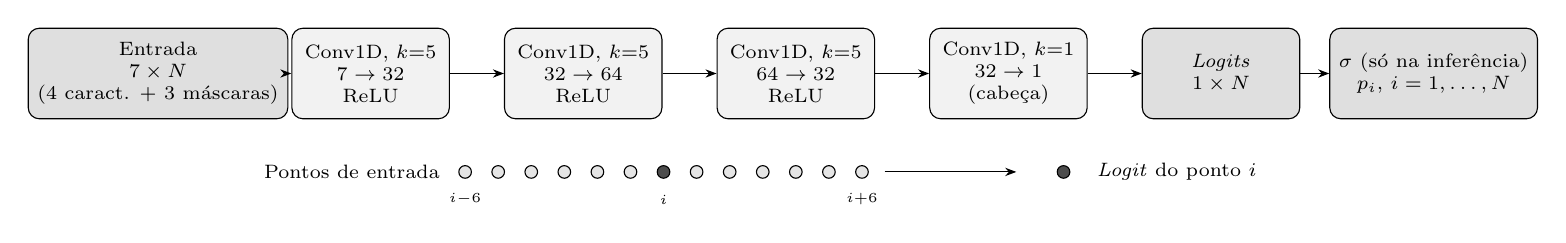
\begin{tikzpicture}[font=\scriptsize, >={Stealth[length=4pt]},
  blk/.style={draw, rounded corners, align=center, minimum height=1.15cm, minimum width=2.0cm, fill=gray!10},
  io/.style={draw, rounded corners, align=center, minimum height=1.15cm, minimum width=2.0cm, fill=gray!25},
  pt/.style={circle, draw, inner sep=0pt, minimum size=0.16cm, fill=gray!20},
  sel/.style={circle, draw, inner sep=0pt, minimum size=0.16cm, fill=black!70}]
\node[io]  (in) at (0,0)    {Entrada\\$7\times N$\\(4 caract. + 3 máscaras)};
\node[blk] (c1) at (2.7,0)  {Conv1D, $k{=}5$\\$7\to32$\\ReLU};
\node[blk] (c2) at (5.4,0)  {Conv1D, $k{=}5$\\$32\to64$\\ReLU};
\node[blk] (c3) at (8.1,0)  {Conv1D, $k{=}5$\\$64\to32$\\ReLU};
\node[blk] (c4) at (10.8,0) {Conv1D, $k{=}1$\\$32\to1$\\(cabeça)};
\node[io]  (z)  at (13.5,0) {\emph{Logits}\\$1\times N$};
\node[io]  (p)  at (16.2,0) {$\sigma$ (só na inferência)\\$p_i$, $i=1,\dots,N$};
\foreach \a/\b in {in/c1,c1/c2,c2/c3,c3/c4,c4/z,z/p}{\draw[->] (\a) -- (\b);}
\foreach \j in {-6,...,6}{
  \pgfmathsetmacro{\xx}{3.9+0.42*(\j+6)}
  \ifnum\j=0 \node[sel] (e\j) at (\xx,-1.25) {};\else\node[pt] (e\j) at (\xx,-1.25) {};\fi}
\node[sel] (o) at (11.5,-1.25) {};
\draw[->] (e6.east) ++(0.2,0) -- (10.9,-1.25);
\node[anchor=east] at (3.7,-1.25) {Pontos de entrada};
\node[anchor=west] at (11.8,-1.25) {\emph{Logit} do ponto $i$};
\node[font=\tiny] at (3.9,-1.6) {$i{-}6$};
\node[font=\tiny] at (6.42,-1.6) {$i$};
\node[font=\tiny] at (8.94,-1.6) {$i{+}6$};
\end{tikzpicture}}
\caption{Em cima, a CNN 1D: o comprimento $N$ mantém-se em todas as camadas. Em baixo, o campo recetivo: cada saída depende dos \resModCampo{} pontos de entrada entre $i-6$ e $i+6$.}
\label{fig:cnn}
\end{figure*}

\textbf{Campo recetivo.} Cada convolução de \emph{kernel} $k$ acrescenta $k-1$ pontos ao contexto, pelo que
\begin{equation}
R = 1+\sum_{j}(k_j-1) = 1+3\times4 = \resModCampo .
\end{equation}
A previsão do ponto $i$ depende dos pontos $i-6,\dots,i+6$ e de mais nenhum. Dar a viagem completa à rede não lhe dá, portanto, contexto global: um comportamento longo só é visto através de vizinhanças locais.

\textbf{Perda.} Usa-se a entropia cruzada binária aplicada aos \emph{logits} (\texttt{BCEWithLogitsLoss}), com média sobre os pontos:
\begin{equation}
\mathcal{L}=-\frac1N\sum_{i=1}^{N}\Big[y_i\log\sigma(z_i)+(1-y_i)\log\big(1-\sigma(z_i)\big)\Big],
\end{equation}
com $y_i=1$ para pesca e $0$ para navegação. Todos os pontos entram na perda. Não há pesos de classe nem reamostragem, pelo que o desequilíbrio entre as classes pode favorecer a maioritária.

\subsection{Janelas e sobreposição}
\label{sec:janelas}

A rede é também treinada e avaliada sobre janelas de $L=\resJZL$ pontos, em duas variantes: \textbf{J0}, sem sobreposição (passo de \resJZPasso{} pontos), e \textbf{J50}, com \resJCSobrep{} de sobreposição (passo de \resJCPasso{} pontos). A sobreposição é a mesma no treino e na inferência. A probabilidade final de cada ponto é a média das probabilidades das janelas que o cobrem; é uma reconstrução e não uma suavização temporal. A rede, os dados, o normalizador e o critério de seleção são os da \emph{baseline}, mas o treino não é igual em tudo: o tamanho do lote e o número de passos também mudam (Tabela~\ref{tab:treino}). O Anexo~\ref{sec:anexo} descreve os pormenores.

\subsection{Filtro temporal}
\label{sec:filtro}

O pós-processamento não volta a treinar a rede. Uma janela de $M=\resPpJanela$ pontos desliza ao longo de cada viagem sobre as probabilidades de pesca, e cada probabilidade é substituída pela média pesada das probabilidades vizinhas:
\begin{equation}
\tilde{p}_i=\frac{\sum_{k=-h}^{h} w_k\,p_{i+k}}{\sum_{k=-h}^{h} w_k},\qquad w_k=\exp\!\left(-\frac{k^2}{2\sigma^2}\right),
\end{equation}
com $h=(M-1)/2$ e $\sigma=M/6\approx\resPpSigma$ pontos. Os pesos gaussianos fazem os vizinhos próximos contar mais do que os afastados (Figura~\ref{fig:janela}, à esquerda). As somas usam só os pontos que existem na viagem, sem pontos inventados e sem atravessar viagens. Depois aplica-se o limiar já fixado do modelo. Filtram-se as probabilidades e não as classes, para que um vizinho previsto com pouca confiança pese menos do que um previsto com muita. Este filtro difere da reconstrução das janelas: esta junta previsões do mesmo ponto, e o filtro junta previsões de pontos vizinhos.

\begin{figure*}[t]
\centering
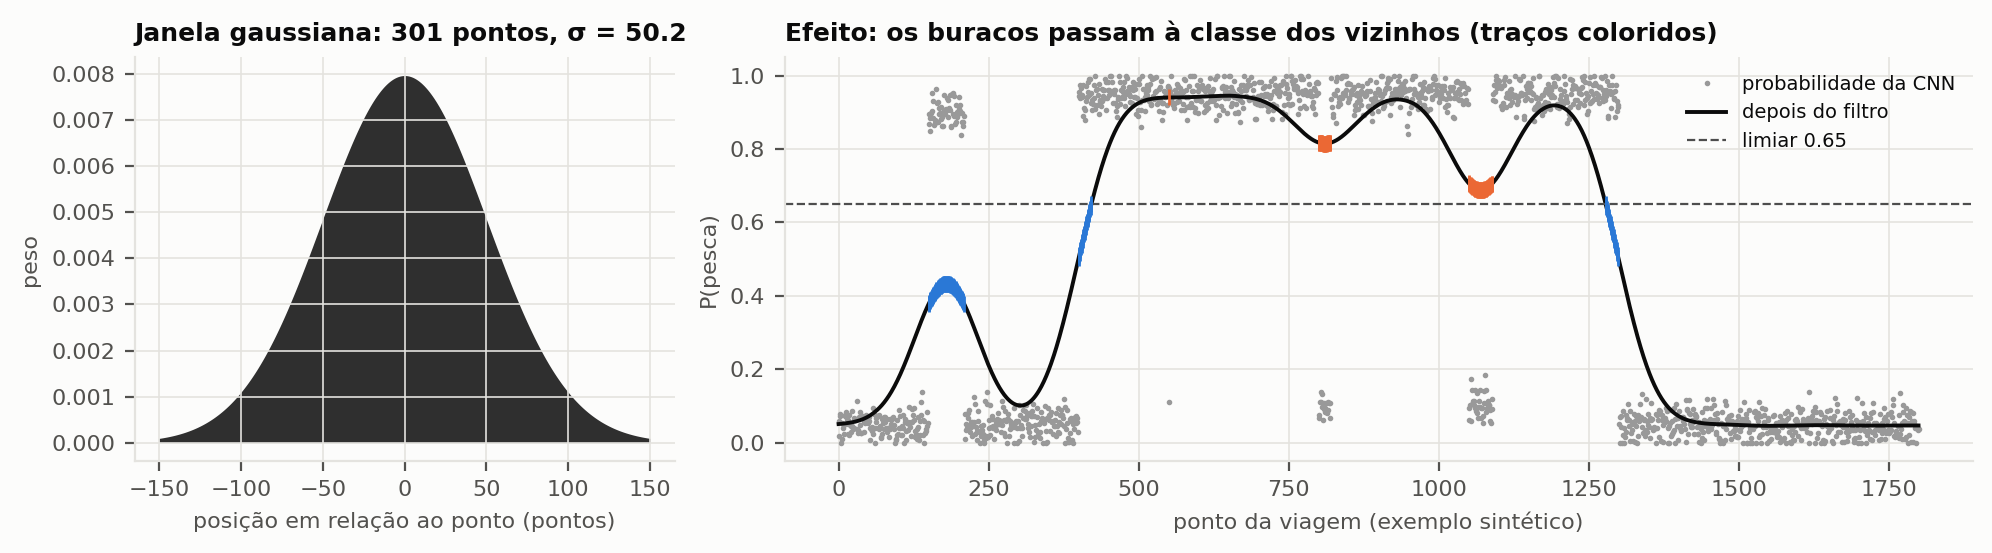
\includegraphics[width=0.85\textwidth]{figures/posproc_janela.png}
\caption{À esquerda, os pesos da janela gaussiana. À direita, um exemplo sintético (não são dados do projeto): blocos de 1, 20 e 40 pontos de navegação no meio da pesca e um bloco de 60 pontos de pesca no meio da navegação passam à classe dos vizinhos (traços coloridos). Nas fronteiras entre blocos longos, o filtro pode deslocar a fronteira.}
\label{fig:janela}
\end{figure*}

\section{Protocolo experimental}
\label{sec:protocolo}

\subsection{Divisão dos dados e papel de cada conjunto}
\label{sec:divisao}

Os dados são divididos por viagem completa (identificador do navio e sufixo da viagem), na proporção 70/15/15, com semente 42 e um manifesto fixo: \resTrViagens{} viagens de treino (\resTrPontos{} pontos), \resSelViagens{} de teste (\resSelPontos{} pontos) e \resVaViagens{} de validação (\resVaPontos{} pontos). Viagens do mesmo navio podem ficar em conjuntos diferentes, por decisão do projeto, pelo que não se afirma generalização a navios inéditos.

Os nomes dos dois conjuntos reservados têm aqui os \textbf{papéis trocados face ao habitual}: o conjunto de \textbf{teste} serve para escolher (épocas, limiares, janela do filtro) e o de \textbf{validação} para a medição final do modelo escolhido. Os resultados no teste são, por isso, otimistas. A preparação das bases leu os três conjuntos, sem analisar resultados; depois dela, cada abertura de um conjunto reservado para escolher ou medir exigiu uma autorização escrita e ficou registada. As anotações da validação foram usadas três vezes para medir: na medição final e, depois, nas duas versões do filtro, sobre as previsões já guardadas e com o protocolo gravado antes de cada uma. Mais tarde serviram também para desenhar figuras, incluindo as da galeria (Anexo~\ref{sec:galeria}), sem escolher nem voltar a ajustar nada.

\subsection{Treino}
\label{sec:treino}

As três experiências usam o otimizador Adam, com taxa de aprendizagem $10^{-3}$ (o valor por omissão, não ajustado), sem decaimento de pesos nem calendário, durante \resTrEpocas{} épocas sem paragem antecipada, e guardam um modelo por época. Partem dos mesmos pesos iniciais (semente \resTrSemente{}) e do mesmo normalizador, ajustado só no treino. A \emph{baseline} usa uma viagem por passo, em ordem aleatória reprodutível, pelo que as viagens longas pesam menos por ponto; J0 e J50 usam lotes de \resJZLote{} janelas e um limite de \resJZOrcamentoMin{} minutos (Tabela~\ref{tab:treino}). Todo o treino foi feito em CPU.

\begin{table}[t]
\centering\footnotesize\setlength{\tabcolsep}{3.5pt}
\begin{tabular}{@{}lrrrr@{}}
\toprule
Modelo & Passo & Janelas & Passos/época & Tempo (min) \\
\midrule
Baseline & --- & (\resTrViagens{} viagens) & \resBsPassos & \resBsSegundos \\
J0 & \resJZPasso & \resJZJanelas & \resJZPassos & \resJZSegundos \\
J50 & \resJCPasso & \resJCJanelas & \resJCPassos & \resJCSegundos \\
\bottomrule
\end{tabular}
\caption{Treino das três experiências (\resTrEpocas{} épocas cada).}
\label{tab:treino}
\end{table}

\subsection{Escolha da época e do limiar}
\label{sec:selecao}

Os critérios foram declarados antes de abrir o conjunto de teste e são iguais para os três modelos: a época com a menor perda por ponto entre as \resSelNCand{} guardadas (nas janelas, calculada depois de reconstruir uma probabilidade por ponto) e, nessa época, o limiar entre \resSelGrelhaMin{} e \resSelGrelhaMax{} (passo 0,05) que maximiza a média dos F1 das duas classes. A \emph{baseline} foi escolhida numa abertura do conjunto de teste, e J0 e J50 numa segunda.

\subsection{Escolha da janela do filtro}
\label{sec:escolha-janela}

Testou-se primeiro um filtro de \resPpViJanela{} pontos, sobre as previsões guardadas da validação. O ganho foi pequeno (Subsecção~\ref{sec:rq2}), pelo que se passou a uma janela maior, de \resPpJanela{} pontos. Este tamanho foi escolhido com o conjunto de teste, sem uma regra declarada antes, a partir da distribuição dos erros da \emph{baseline} e do cálculo aproximado descrito abaixo; o efeito no teste, comparado com o de outras dimensões, só foi medido depois da escolha. Um \emph{bloco de erro} é uma sequência de pontos seguidos mal classificados com a mesma classe prevista. No teste há \resBuTesteBlocos{} blocos, que somam \resBuTesteErros{} pontos errados, com mediana de \resBuTesteMediana{} pontos, média de \resBuTesteMedia{}, 90\,\% até \resBuTesteNoventa{} pontos e um máximo de \resBuTesteMaximo{}. A navegação prevista no meio da pesca representa \resBuTesteNavPercPontos{} dos pontos errados.

Como o limiar do modelo (\resSelLimiar{}) não está a meio da escala, o filtro é assimétrico. Num cálculo com probabilidades ideais (0 ou 1), uma janela de \resPpJanela{} pontos remove blocos isolados de pesca até \resBuRemovePesca{} pontos e de navegação até \resBuRemoveNav{}. Por este critério aproximado, abrange \resBuTesteBlocosCobertos{} dos blocos do teste, mas só \resBuTestePontosCobertos{} dos pontos errados, porque os blocos longos concentram muitos erros. O segmento real de navegação mais curto tem \resBuTreinoRealNavMin{} pontos no treino e \resBuTesteRealNavMin{} no teste, acima do que o filtro remove.

\subsection{Métricas}
\label{sec:metricas}

\textbf{Por ponto:} exatidão, precisão, sensibilidade, F1 e \emph{intersection-over-union} (IoU) de cada classe, comparadas com a regra que prevê sempre a classe maioritária.

\textbf{Por segmento:} um segmento é um bloco máximo de pontos seguidos da mesma classe numa viagem, extraído sem suavizar. Um segmento previsto corresponde a um real da mesma classe quando o IoU temporal, em segundos, é de pelo menos 0,5, com correspondência um-para-um, começando pelos pares de maior IoU. Mede-se o F1 de segmentos, a \emph{fragmentação} (segmentos previstos a dividir pelos reais; o valor 1 indica o mesmo número) e o \emph{erro de fronteira} (mediana do desvio absoluto, no início e no fim, nos pares correspondidos).

\subsection{Medições no conjunto de validação}
\label{sec:medicoes}

\textbf{Medição final.} Antes de abrir o conjunto, mas já conhecidos os resultados dos três modelos no teste, declarou-se que se mediria só o modelo com o maior F1 médio por ponto no teste, com a exatidão a desempatar. Foi a \emph{baseline} (F1 médio de \resVaFMedioBs{}, contra \resVaFMedioJC{} de J50 e \resVaFMedioJZ{} de J0). O conjunto foi aberto uma vez, com o modelo, a época (\resVaEpoca{}) e o limiar (\resVaLimiar{}) fixados.

\textbf{Pós-processamento.} O filtro aplicou-se às probabilidades guardadas nessa medição, sem voltar a ler os dados nem a correr a CNN, e comparou-se com as anotações antes e depois. O protocolo da versão de \resPpJanela{} pontos (houve uma anterior; Secção~\ref{sec:limitacoes}) foi gravado num \emph{commit} antes da execução, e uma segunda implementação confirmou os números. Esta medição não é independente (Secção~\ref{sec:limitacoes}).

\subsection{Reprodutibilidade e verificação}

O código foi verificado com testes automáticos sobre dados sintéticos (e, para a leitura das sequências, sobre três viagens de treino): alinhamento entre previsão e ponto, separação das viagens, valores em falta, ausência de vazamento para a normalização, recusa dos conjuntos reservados no desenvolvimento, campo recetivo, perda e gradientes, cobertura e reconstrução das janelas, métricas e filtro. Estes testes verificam o código e não a qualidade do modelo. Registam-se a semente, as versões (PyTorch \resTrTorch{}), o normalizador e os \emph{hashes} dos ficheiros, sem garantia de resultados idênticos entre máquinas. Os números deste relatório provêm de ficheiros de resultados gerados por código.

\section{Resultados e discussão}
\label{sec:resultados}

\subsection{Janelas e sobreposição (RQ1)}
\label{sec:rq1}

Esta comparação usa o conjunto de teste, que serviu para escolher a época e o limiar de cada modelo.

\textbf{Por segmento}, os três modelos fragmentam muito (Tabela~\ref{tab:segmentos}): há \resBsSegPescaNRef{} segmentos reais de pesca, e a \emph{baseline} prevê \resBsSegPescaNPred{}, J0 \resJZSegPescaNPred{} e J50 \resJCSegPescaNPred{}. A fragmentação de J50 é a menor (na pesca, \resJCSegPescaFrag{} contra \resJZSegPescaFrag{} de J0 e \resBsSegPescaFrag{} da \emph{baseline}; na navegação, \resJCSegNavFrag{} contra \resJZSegNavFrag{} e \resBsSegNavFrag{}), mas continua muito acima de 1. O F1 de segmentos de pesca é muito baixo nos três, sobretudo porque há centenas de segmentos previstos para poucos reais (na \emph{baseline}, a precisão por segmento é de \resBsSegPescaPrec{}); além disso, há em média um segmento real de pesca por viagem, e um previsto só lhe corresponde se o IoU temporal chegar ao limiar. O erro de fronteira da pesca não mostra um padrão e assenta em poucos pares (\resBsSegPescaNPar{}, \resJZSegPescaNPar{} e \resJCSegPescaNPar{}). A Figura~\ref{fig:linha} mostra a viagem de teste com mais segmentos reais. Todas as viagens estão na galeria do Anexo~\ref{sec:galeria}.

\begin{table*}[t]
\centering\footnotesize\setlength{\tabcolsep}{4pt}
\begin{tabular}{@{}llrrrrrrr@{}}
\toprule
Modelo & Classe & Reais & Previstos & Pares & F1 & Fragm. & Erro início (s) & Erro fim (s) \\
\midrule
Baseline & Pesca & \resBsSegPescaNRef & \resBsSegPescaNPred & \resBsSegPescaNPar & \resBsSegPescaF & \resBsSegPescaFrag & \resBsSegPescaIniMed & \resBsSegPescaFimMed \\
J0 & Pesca & \resJZSegPescaNRef & \resJZSegPescaNPred & \resJZSegPescaNPar & \resJZSegPescaF & \resJZSegPescaFrag & \resJZSegPescaIniMed & \resJZSegPescaFimMed \\
J50 & Pesca & \resJCSegPescaNRef & \resJCSegPescaNPred & \resJCSegPescaNPar & \resJCSegPescaF & \resJCSegPescaFrag & \resJCSegPescaIniMed & \resJCSegPescaFimMed \\
\midrule
Baseline & Navegação & \resBsSegNavNRef & \resBsSegNavNPred & \resBsSegNavNPar & \resBsSegNavF & \resBsSegNavFrag & \resBsSegNavIniMed & \resBsSegNavFimMed \\
J0 & Navegação & \resJZSegNavNRef & \resJZSegNavNPred & \resJZSegNavNPar & \resJZSegNavF & \resJZSegNavFrag & \resJZSegNavIniMed & \resJZSegNavFimMed \\
J50 & Navegação & \resJCSegNavNRef & \resJCSegNavNPred & \resJCSegNavNPar & \resJCSegNavF & \resJCSegNavFrag & \resJCSegNavIniMed & \resJCSegNavFimMed \\
\bottomrule
\end{tabular}
\caption{Métricas por segmento no conjunto de teste. ``Pares'' são os segmentos correspondidos (IoU temporal $\geq$ 0,5), ``Fragm.'' a razão previstos/reais, e os erros de fronteira são medianas nos pares.}
\label{tab:segmentos}
\end{table*}

\begin{figure*}[t]
\centering
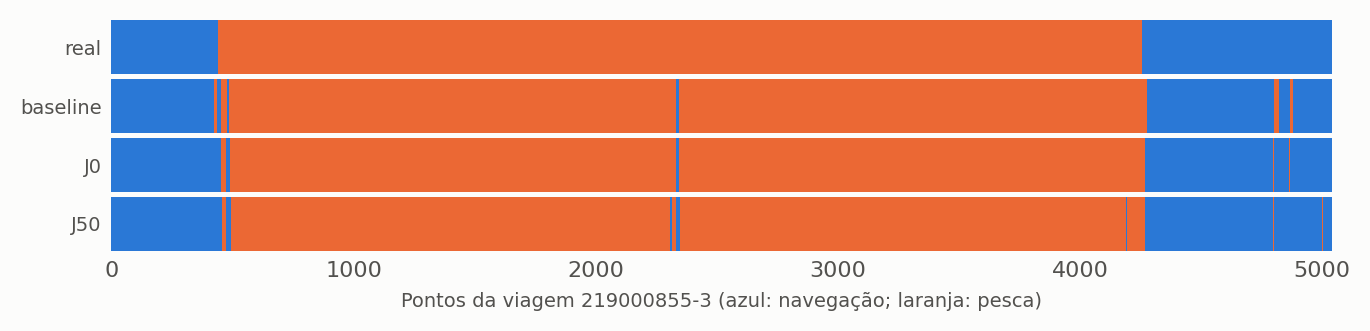
\includegraphics[width=0.85\textwidth]{figures/janelas_linha_temporal_baseline.png}
\caption{Uma viagem do conjunto de teste: classe real e classe prevista pela \emph{baseline}, por J0 e por J50, ponto a ponto.}
\label{fig:linha}
\end{figure*}

\textbf{Por ponto}, nenhuma variante com janelas supera a \emph{baseline} em exatidão (Tabela~\ref{tab:pontos}). Face a ela, J0 tem exatidão maior em \resJZViagMelhor{} viagens e menor em \resJZViagPior{} (diferença mediana de \ptnum{\resJZViagDifMed} pontos percentuais), e J50 maior em \resJCViagMelhor{} e menor em \resJCViagPior{} (\ptnum{\resJCViagDifMed}). A \emph{baseline} acerta mais na navegação (sensibilidade de \resBsTesteNavSens{}, contra \resJZTesteNavSens{} e \resJCTesteNavSens{}) e tem melhor precisão na pesca (\resBsTestePescaPrec{}, contra \resJZTestePescaPrec{} e \resJCTestePescaPrec{}). Por viagem, o valor mais baixo é de J0, que desce a \resJZTesteViagMin{}, quando a \emph{baseline} não desce abaixo de \resTesteViagMin{} (Figura~\ref{fig:viagens}). As métricas por classe estão no Anexo~\ref{sec:anexo}.

\begin{table}[t]
\centering\footnotesize\setlength{\tabcolsep}{3.5pt}
\begin{tabular}{@{}lrrrrrr@{}}
\toprule
Modelo & Época & Limiar & Treino & Teste & F1 nav. & F1 pesca \\
\midrule
Baseline & \resBsEpoca & \resBsLimiar & \resBsTreinoAcc & \resBsTesteAcc & \resBsTesteNavF & \resBsTestePescaF \\
J0 & \resJZEpoca & \resJZLimiar & \resJZTreinoAcc & \resJZTesteAcc & \resJZTesteNavF & \resJZTestePescaF \\
J50 & \resJCEpoca & \resJCLimiar & \resJCTreinoAcc & \resJCTesteAcc & \resJCTesteNavF & \resJCTestePescaF \\
\bottomrule
\end{tabular}
\caption{Resumo por ponto: época e limiar escolhidos, exatidão no treino e no teste e F1 por classe no teste. A regra da classe maioritária dá \resBsTreinoAccMaj{} no treino e \resBsTesteAccMaj{} no teste.}
\label{tab:pontos}
\end{table}

\begin{figure*}[t]
\centering
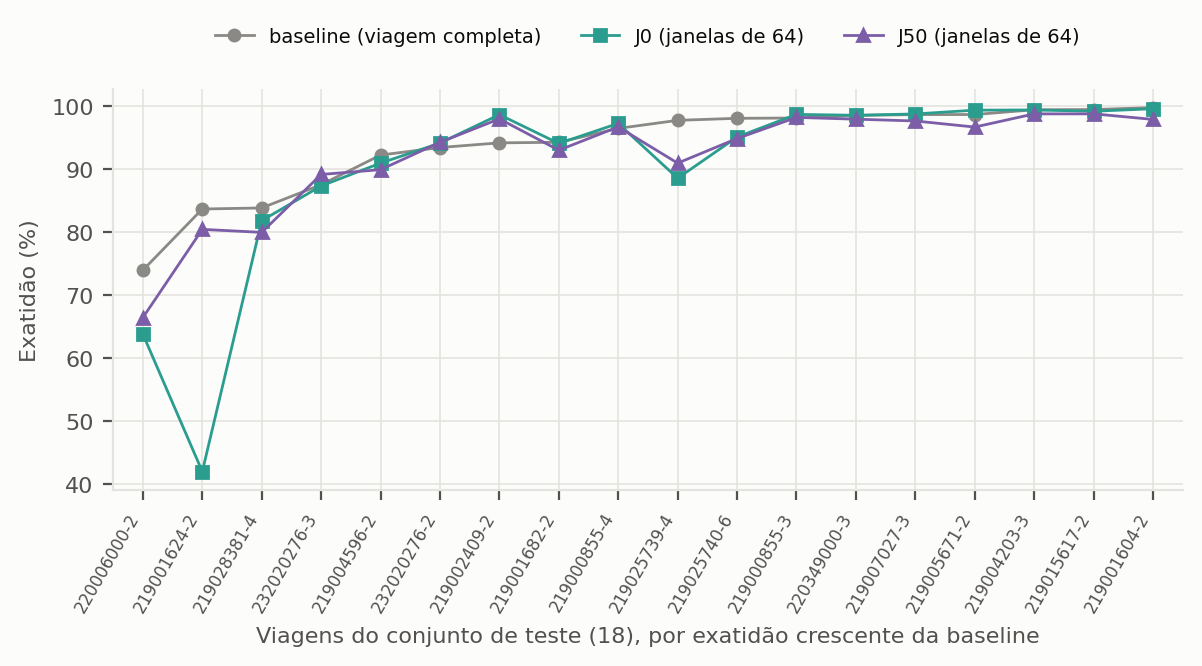
\includegraphics[width=0.75\textwidth]{figures/janelas_viagens_baseline.png}
\caption{Exatidão por viagem no conjunto de teste, com as viagens ordenadas pela exatidão da \emph{baseline}.}
\label{fig:viagens}
\end{figure*}

\textbf{Épocas escolhidas.} J0 e J50 ficam nas épocas \resJZEpoca{} e \resJCEpoca{}, muito antes da época \resBsEpoca{} da \emph{baseline}, porque a sua perda no teste sobe com o treino enquanto a do treino desce (Figura~\ref{fig:perda}), o que é compatível com ajuste excessivo às viagens de treino. Na \emph{baseline} a perda no teste oscila entre épocas, pelo que também a sua escolha é sensível a essa oscilação.

\begin{figure*}[t]
\centering
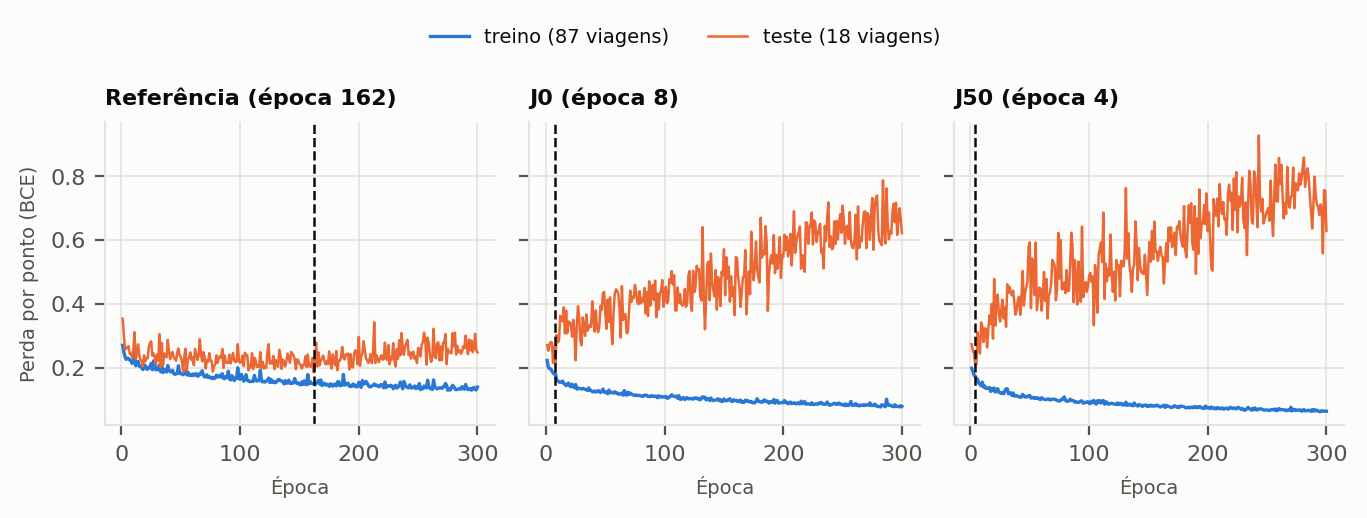
\includegraphics[width=0.85\textwidth]{figures/janelas_perda.png}
\caption{Perda por ponto ao longo das épocas, nas viagens de treino e nas de teste. A linha tracejada marca a época escolhida.}
\label{fig:perda}
\end{figure*}

\textbf{Resposta à RQ1.} Neste conjunto, J50 fragmenta menos do que J0 e do que a \emph{baseline}, mas não melhora o erro de fronteira da pesca de forma consistente. Por ponto, J50 fica ligeiramente acima de J0 (\resJCTesteAcc{} contra \resJZTesteAcc{}) e abaixo da \emph{baseline} (\resBsTesteAcc{}); com uma só semente, a diferença entre J0 e J50 não permite concluir. J0 não supera a \emph{baseline}, e J50 troca menos fragmentos por menor exatidão: não se conclui que o janelamento ou a sobreposição melhorem a segmentação. A instabilidade das fronteiras é aqui avaliada pela fragmentação e pelo erro de fronteira. Como J50 e J0 diferem também no limiar (\resJCLimiar{} e \resJZLimiar{}), na época e no número de passos (J50 faz \resJCPassosVezes{} vezes os de J0), a diferença de fragmentação não se pode atribuir só à sobreposição.

\subsection{Medição final da \emph{baseline}}
\label{sec:validacao}

No conjunto de validação, a exatidão por ponto é de \resVaValidAcc{} (\resVaValidErros{} erros em \resVaValidPontos{} pontos), contra \resVaValidAccMaj{} da regra da classe maioritária (pesca, \resVaPercPesca{} dos pontos). No teste, a mesma rede tem \resVaTesteAcc{}, contra \resVaTesteAccMaj{}; como a proporção de pesca é muito diferente entre os conjuntos, as exatidões não são diretamente comparáveis. A pesca é bem detetada (Tabela~\ref{tab:validacao}), mas a precisão da navegação desce para \resVaValidNavPrec{} (\resVaTesteNavPrec{} no teste): há \resVaValidFN{} pontos de pesca previstos como navegação, contra \resVaValidTN{} pontos de navegação certos, e a navegação é a classe minoritária.

\begin{table}[t]
\centering\footnotesize\setlength{\tabcolsep}{3.5pt}
\begin{tabular}{@{}llrrrrr@{}}
\toprule
Conjunto & Classe & Pontos & Prec. & Sensib. & F1 & IoU \\
\midrule
Validação & Navegação & \resVaValidNavReal & \resVaValidNavPrec & \resVaValidNavSens & \resVaValidNavF & \resVaValidNavIoU \\
Validação & Pesca & \resVaValidPescaReal & \resVaValidPescaPrec & \resVaValidPescaSens & \resVaValidPescaF & \resVaValidPescaIoU \\
Teste & Navegação & \resVaTesteNavReal & \resVaTesteNavPrec & \resVaTesteNavSens & \resVaTesteNavF & \resVaTesteNavIoU \\
Teste & Pesca & \resVaTestePescaReal & \resVaTestePescaPrec & \resVaTestePescaSens & \resVaTestePescaF & \resVaTestePescaIoU \\
\bottomrule
\end{tabular}
\caption{\emph{Baseline} por ponto: medição final (validação) e, para comparação, teste (otimista).}
\label{tab:validacao}
\end{table}

Por viagem, a exatidão vai de \resVaViagMin{} (viagem \resVaPiorViagem) a \resVaViagMax{}, com mediana de \resVaViagMed{}. O número de viagens em que o modelo não supera a regra da classe maioritária da própria viagem é \resVaNViagNaoSuperam{}. Na pior viagem, o modelo passa a prever quase só navegação a meio do segmento real de pesca (Figura~\ref{fig:validacao}). Por segmento, a fragmentação é grande: \resVaSegPescaNPred{} segmentos de pesca previstos para \resVaSegPescaNRef{} reais (linhas ``antes'' da Tabela~\ref{tab:filtro}).

\begin{figure*}[t]
\centering
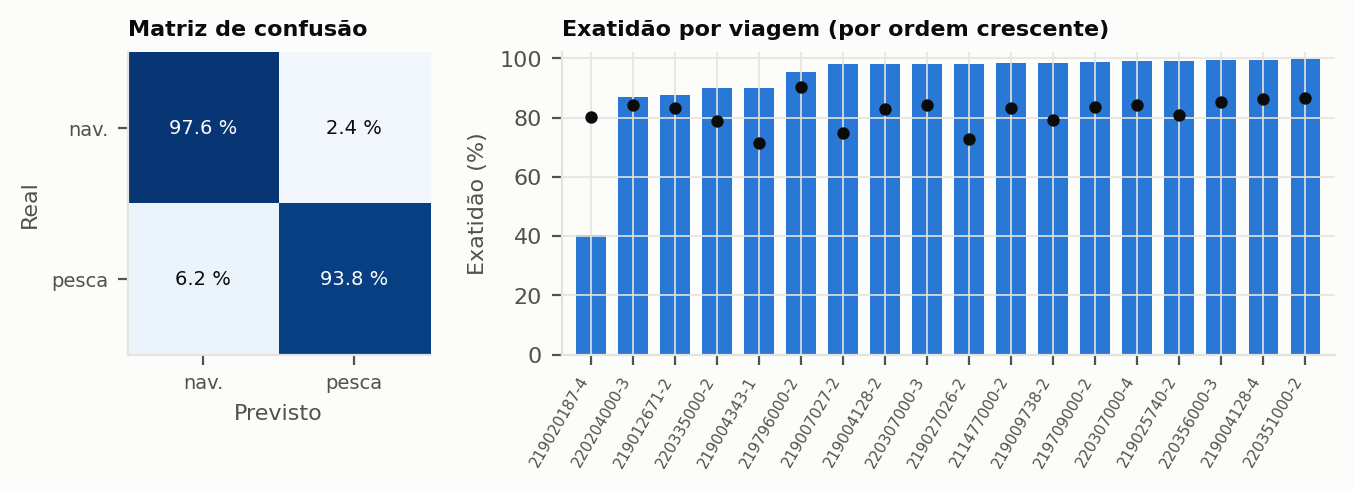
\includegraphics[width=0.8\textwidth]{figures/validacao_resumo.png}\\[2pt]
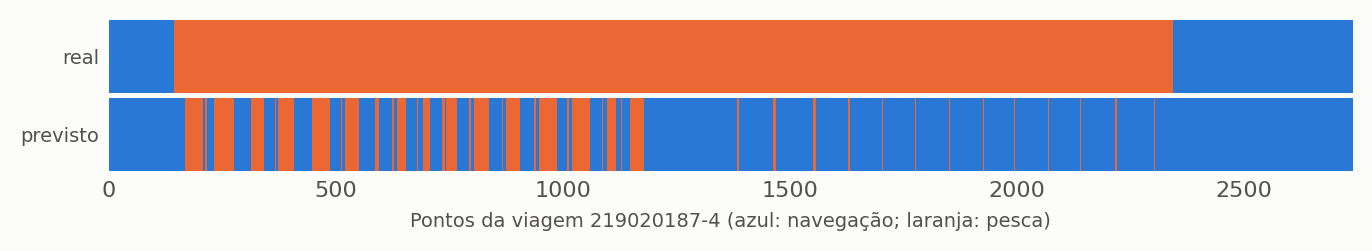
\includegraphics[width=0.8\textwidth]{figures/validacao_pior_viagem.png}
\caption{Medição final. Em cima, matriz de confusão por ponto (percentagem da classe real prevista em cada classe) e exatidão por viagem (os pontos pretos indicam a regra da classe maioritária de cada viagem). Em baixo, a viagem de menor exatidão.}
\label{fig:validacao}
\end{figure*}

% A Figura 8 está antes da subsecção que a cita para sair antes dos anexos (REV-080).
\begin{figure*}[t]
\centering
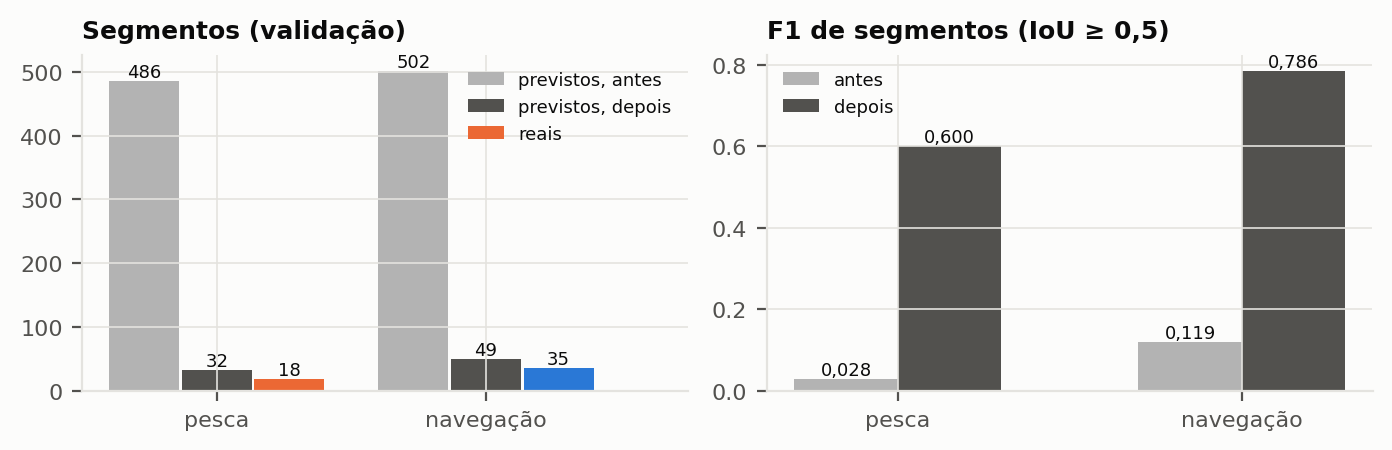
\includegraphics[width=0.75\textwidth]{figures/posproc_resultados.png}\\[2pt]
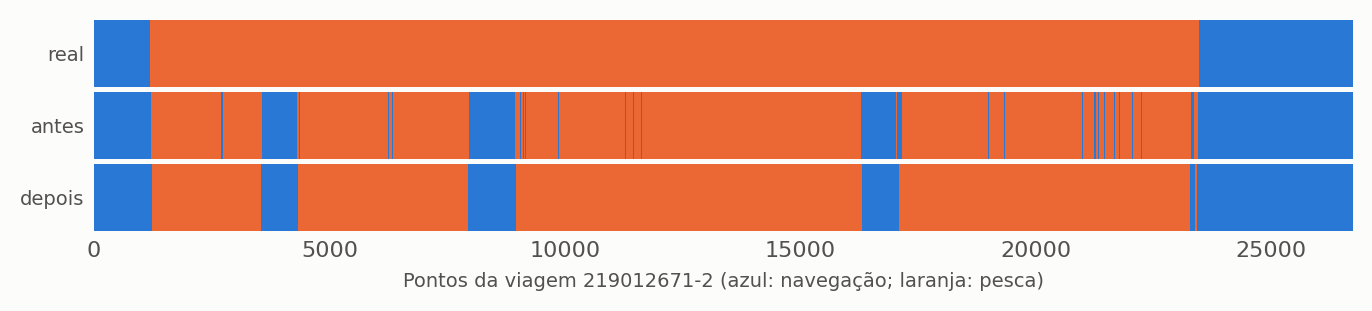
\includegraphics[width=0.85\textwidth]{figures/posproc_viagem.png}
\caption{Efeito do filtro no conjunto de validação. Em cima, segmentos previstos e F1 de segmentos. Em baixo, a viagem com mais segmentos de pesca previstos antes do filtro: as interrupções curtas desaparecem e os blocos longos de erro ficam.}
\label{fig:filtro}
\end{figure*}

\subsection{Filtro temporal (RQ2)}
\label{sec:rq2}

Com a primeira janela, de \resPpViJanela{} pontos, o ganho foi pequeno: a exatidão por ponto passou de \resPpAntesAcc{} para \resPpViDepoisAcc{}, os segmentos de pesca previstos de \resPpASegPescaNPred{} para \resPpViSegPescaNPred{} (reais: \resPpASegPescaNRef{}) e o F1 de segmentos de pesca de \resPpASegPescaF{} para \resPpViSegPescaF{}, melhorando \resPpViViagMelhoram{} viagens e piorando \resPpViViagPioram{}. Os resultados seguintes são os da janela de \resPpJanela{} pontos.

O filtro muda a classe de \resPpMudam{} pontos (\resPpPercMudam{}): \resPpCorrigidos{} passam a estar certos e \resPpEstragados{} passam a estar errados, ou seja, há \resPpErrosMenos{} erros a menos. A exatidão por ponto passa de \resPpAntesAcc{} para \resPpDepoisAcc{}. O efeito principal está nos segmentos (Tabela~\ref{tab:filtro} e Figura~\ref{fig:filtro}): os de pesca previstos descem de \resPpASegPescaNPred{} para \resPpDSegPescaNPred{} (reais: \resPpASegPescaNRef{}) e os de navegação de \resPpASegNavNPred{} para \resPpDSegNavNPred{} (reais: \resPpASegNavNRef{}), e o F1 de segmentos sobe nas duas classes. Os erros de fronteira também descem ou mantêm-se, mas as medianas calculam-se sobre os pares correspondidos, que mudam (na pesca, de \resPpASegPescaNPar{} para \resPpDSegPescaNPar{}), pelo que o antes e o depois não comparam os mesmos segmentos.

\begin{table*}[t]
\centering\footnotesize\setlength{\tabcolsep}{4pt}
\begin{tabular}{@{}llrrrrrrr@{}}
\toprule
Classe & Filtro & F1 (ponto) & Previstos & Pares & F1 (segm.) & Fragm. & Erro início (s) & Erro fim (s) \\
\midrule
Pesca & Antes & \resPpAntesPescaF & \resPpASegPescaNPred & \resPpASegPescaNPar & \resPpASegPescaF & \resPpASegPescaFrag & \resPpASegPescaIniMed & \resPpASegPescaFimMed \\
Pesca & Depois & \resPpDepoisPescaF & \resPpDSegPescaNPred & \resPpDSegPescaNPar & \resPpDSegPescaF & \resPpDSegPescaFrag & \resPpDSegPescaIniMed & \resPpDSegPescaFimMed \\
\midrule
Navegação & Antes & \resPpAntesNavF & \resPpASegNavNPred & \resPpASegNavNPar & \resPpASegNavF & \resPpASegNavFrag & \resPpASegNavIniMed & \resPpASegNavFimMed \\
Navegação & Depois & \resPpDepoisNavF & \resPpDSegNavNPred & \resPpDSegNavNPar & \resPpDSegNavF & \resPpDSegNavFrag & \resPpDSegNavIniMed & \resPpDSegNavFimMed \\
\bottomrule
\end{tabular}
\caption{\emph{Baseline} no conjunto de validação antes e depois do filtro de \resPpJanela{} pontos. Segmentos reais: \resPpASegPescaNRef{} de pesca e \resPpASegNavNRef{} de navegação.}
\label{tab:filtro}
\end{table*}

O efeito não é igual em todas as viagens: das \resPpNViagens{}, melhoram \resPpViagMelhoram{} e pioram \resPpViagPioram{}. A maior queda é na viagem \resPpPiorQuedaViagem{}, de \resPpPiorQuedaAntes{} para \resPpPiorQuedaDepois{}, a mesma que já tinha a menor exatidão: quando a CNN erra durante muito tempo, o filtro pode alargar o erro em vez de o corrigir. Blocos de erro maiores do que o filtro consegue remover podem ficar, e um segmento real mais curto do que esses limites pode ser apagado.

\textbf{Resposta à RQ2.} Neste conjunto, o filtro reduz muito a fragmentação e aproxima os segmentos previstos dos anotados; a exatidão por ponto sobe pouco. É um resultado a confirmar em dados novos, porque a medição não é independente (Secção~\ref{sec:limitacoes}).

\subsection{Interação entre sobreposição e filtro (RQ3)}
\label{sec:rq3}

A RQ3 fica \textbf{sem resposta}. Medir a interação exige comparar as quatro combinações (sem e com sobreposição, sem e com filtro) nas mesmas condições:
\begin{itemize}
\item só a \emph{baseline} foi filtrada; J0 e J50 nunca o foram;
\item não há um conjunto limpo onde medir: a validação já foi usada, e foi no teste que se escolheram as épocas, os limiares e a janela, esta a partir dos erros da \emph{baseline}, o que enviesaria a comparação a favor dela;
\item J0 e J50 foram escolhidas em épocas muito precoces e treinadas com lotes e números de passos diferentes dos da \emph{baseline};
\item os dois efeitos sobrepõem-se: a média das janelas já suaviza um pouco as previsões, e o filtro muito mais. É plausível que a vantagem da sobreposição desapareça depois do filtro, mas isso é uma hipótese e não um resultado.
\end{itemize}
Responder-lhe exigiria um desenho fatorial planeado de início, com o mesmo critério de seleção, várias sementes e um conjunto final ainda por abrir.

\section{Limitações, ética e dimensão humana}
\label{sec:limitacoes}

\textbf{Limitações dos resultados.}
\begin{itemize}
\item \textbf{Filtro.} Antes desta versão, foi medido no conjunto de validação um filtro com uma janela de 13 pontos; a decisão de procurar outra janela foi tomada depois de ver esse resultado. O valor obtido com \resPpJanela{} pontos não é, por isso, uma medição final independente.
\item \textbf{Teste otimista.} O conjunto de teste serviu para escolher épocas, limiares e a janela; a comparação entre a \emph{baseline}, J0 e J50 assenta só nele.
\item \textbf{Treinos não equivalentes.} As variantes com janelas diferem da \emph{baseline} no lote e no número de passos, e ficaram em épocas muito anteriores.
\item \textbf{Poucos dados.} Uma só semente, \resVaViagens{} viagens em cada conjunto reservado e sem intervalos de incerteza.
\item \textbf{Navios.} A divisão é por viagem, pelo que não se afirma generalização a navios inéditos.
\item \textbf{Um só contexto.} Os dados cobrem uma semana de navios de pesca em águas dinamarquesas (Secção~\ref{sec:dados}); não se sabe como o modelo se comporta noutras regiões ou épocas. As anotações são manuais e não se conhece uma medida da sua fiabilidade.
\item \textbf{Modelo.} A arquitetura e a taxa de aprendizagem não foram otimizadas, e o campo recetivo (\resModCampo{} pontos) é muito menor do que os blocos de erro mais longos.
\end{itemize}

\textbf{Ética.} Detetar um comportamento compatível com pesca não demonstra ilegalidade: o modelo não verifica licenças, quotas, zonas autorizadas nem infrações. Apesar de os dados serem públicos, a deteção automática não deve, por si só, fundamentar sanções; a decisão tem de ser humana. Um sistema em uso teria de ser transparente e de verificar se erra mais para certos tipos de navio, regiões ou comunidades de pesca, o que não foi avaliado.

\textbf{Dimensão humana.} Para apoiar o inspetor estavam previstas a explicabilidade, através de atribuições de importância~\cite{lundberg2017}, a confiança calibrada~\cite{guo2017} e um \emph{dashboard} de prova de conceito. Estas partes não foram concluídas nesta fase. A probabilidade devolvida pela CNN não é uma confiança calibrada e não deve ser apresentada como tal, e sem um estudo com inspetores não se pode afirmar utilidade operacional.

\section{Conclusões e trabalho futuro}
\label{sec:conclusoes}
Este trabalho comparou uma CNN 1D aplicada à viagem completa com a mesma rede aplicada a janelas e estudou um filtro temporal sobre as previsões da \emph{baseline}.

\textbf{RQ1.} No teste, J50 prevê menos segmentos de pesca do que J0 (\resJCSegPescaNPred{} contra \resJZSegPescaNPred{}; a \emph{baseline}, \resBsSegPescaNPred{}), embora os dois também difiram no limiar, na época e no número de passos, sem melhorar de forma consistente o erro de fronteira, e nenhuma variante com janelas supera a exatidão da \emph{baseline} (\resBsTesteAcc{}, contra \resJCTesteAcc{} de J50). Não há base para concluir que as janelas melhorem a segmentação.

\textbf{RQ2.} Neste conjunto, o filtro reduz os segmentos de pesca previstos de \resPpASegPescaNPred{} para \resPpDSegPescaNPred{} (reais: \resPpASegPescaNRef{}) e sobe o F1 de segmentos de pesca de \resPpASegPescaF{} para \resPpDSegPescaF{}, com a exatidão por ponto a passar de \resPpAntesAcc{} para \resPpDepoisAcc{}. A medição não é independente e falta confirmá-la em dados novos.

\textbf{RQ3.} Fica sem resposta (Subsecção~\ref{sec:rq3}).

\textbf{Critérios de sucesso.} O critério (i) cumpre-se com ressalvas: o efeito das janelas foi medido só no teste e o do filtro numa medição não independente. O (ii) cumpre-se em parte: a segmentação fica muito menos fragmentada, mas a fragmentação continua acima de 1 (\resPpDSegPescaFrag{} na pesca e \resPpDSegNavFrag{} na navegação), há erros longos, e a estabilidade perante pequenas alterações não foi medida. O (iii) não se cumpre.

\textbf{Trabalho futuro.} Concluir o apoio à decisão previsto (Secção~\ref{sec:limitacoes}); dar mais contexto à CNN; estudar o limiar em conjunto com o filtro; testar mais dimensões da janela do filtro, maiores e menores, e outros tipos de janela, para perceber como mudam os resultados; confirmar o filtro em dados novos; repetir com várias sementes e uma divisão por navio; e responder à RQ3 com um desenho fatorial.

\appendix
\raggedbottom

\section{Anexo: pormenores do janelamento}
\label{sec:anexo}

\textbf{Janelas.} Cada viagem começa no primeiro ponto e avança pelo passo até uma janela alcançar o fim. Nenhuma janela mistura viagens, mas, dentro de uma viagem, atravessam os intervalos de tempo, tal como a \emph{baseline} trata a viagem como uma só sequência. A última janela pode ficar mais curta do que $L$ (\resJZJanelasCurtas{} janelas curtas em J0 e \resJCJanelasCurtas{} em J50), sem pontos falsos, e uma viagem com no máximo $L$ pontos dá uma só janela.

\textbf{Lotes e perda.} Para juntar janelas de comprimentos diferentes num lote usa-se um enchimento, que a perda ignora e que a rede volta a pôr a zero na entrada e depois de cada ReLU; a previsão de uma janela curta é assim a que teria sozinha. A perda do lote é a média sobre as posições reais, pelo que um ponto presente em duas janelas conta duas vezes.

\textbf{Reconstrução.} A probabilidade de cada ponto é a média simples das probabilidades das janelas que o cobrem, calculada em precisão dupla, e só depois se aplica o limiar. A perda usada para escolher a época calcula-se sobre essa probabilidade, com um recorte de $10^{-12}$.

\par\noindent\begin{minipage}{\columnwidth}
\begin{center}
\scriptsize\setlength{\tabcolsep}{2.2pt}
\begin{tabular}{@{}lllrrrrr@{}}
\toprule
Modelo & Conjunto & Classe & Pontos & Prec. & Sensib. & F1 & IoU \\
\midrule
Base & Treino & Nav. & \resBsTreinoNavReal & \resBsTreinoNavPrec & \resBsTreinoNavSens & \resBsTreinoNavF & \resBsTreinoNavIoU \\
Base & Treino & Pesca & \resBsTreinoPescaReal & \resBsTreinoPescaPrec & \resBsTreinoPescaSens & \resBsTreinoPescaF & \resBsTreinoPescaIoU \\
Base & Teste & Nav. & \resBsTesteNavReal & \resBsTesteNavPrec & \resBsTesteNavSens & \resBsTesteNavF & \resBsTesteNavIoU \\
Base & Teste & Pesca & \resBsTestePescaReal & \resBsTestePescaPrec & \resBsTestePescaSens & \resBsTestePescaF & \resBsTestePescaIoU \\
J0 & Treino & Nav. & \resJZTreinoNavReal & \resJZTreinoNavPrec & \resJZTreinoNavSens & \resJZTreinoNavF & \resJZTreinoNavIoU \\
J0 & Treino & Pesca & \resJZTreinoPescaReal & \resJZTreinoPescaPrec & \resJZTreinoPescaSens & \resJZTreinoPescaF & \resJZTreinoPescaIoU \\
J0 & Teste & Nav. & \resJZTesteNavReal & \resJZTesteNavPrec & \resJZTesteNavSens & \resJZTesteNavF & \resJZTesteNavIoU \\
J0 & Teste & Pesca & \resJZTestePescaReal & \resJZTestePescaPrec & \resJZTestePescaSens & \resJZTestePescaF & \resJZTestePescaIoU \\
J50 & Treino & Nav. & \resJCTreinoNavReal & \resJCTreinoNavPrec & \resJCTreinoNavSens & \resJCTreinoNavF & \resJCTreinoNavIoU \\
J50 & Treino & Pesca & \resJCTreinoPescaReal & \resJCTreinoPescaPrec & \resJCTreinoPescaSens & \resJCTreinoPescaF & \resJCTreinoPescaIoU \\
J50 & Teste & Nav. & \resJCTesteNavReal & \resJCTesteNavPrec & \resJCTesteNavSens & \resJCTesteNavF & \resJCTesteNavIoU \\
J50 & Teste & Pesca & \resJCTestePescaReal & \resJCTestePescaPrec & \resJCTestePescaSens & \resJCTestePescaF & \resJCTestePescaIoU \\
\bottomrule
\end{tabular}
\captionof{table}{Métricas por ponto e por classe no treino e no teste. Os valores do teste são otimistas, porque este conjunto serviu para escolher as épocas e os limiares. Base: \emph{baseline}.}
\label{tab:classes}
\end{center}
\end{minipage}

\section{Anexo: galeria de viagens}
\label{sec:galeria}

A galeria mostra, viagem a viagem, a classe real e a prevista em cada ponto: nas \resSelViagens{} viagens de teste, pela \emph{baseline}, por J0, por J50 e pela \emph{baseline} com o filtro; nas \resVaViagens{} de validação, pela \emph{baseline} sem e com o filtro. Cada viagem traz a exatidão e o número de segmentos de pesca. Foi gerada a partir das previsões guardadas, só para consulta, e valem as ressalvas da Secção~\ref{sec:limitacoes}. O PDF está no repositório do projeto:

{\small\urlstyle{tt}\url{https://github.com/DinisRosa/IACH-AIS-Project_4/blob/main/viagens/galeria_viagens.pdf}}

% As figuras pendentes ficam antes das referências; o anexo corre logo a seguir às conclusões (REV-071).
\FloatBarrier
\bibliographystyle{FormattingGuidelines-IJCAI-ECAI-26/named}
\bibliography{references}

\end{document}
